%
%   This file is part of the APS files in the REVTeX 4 distribution.
%   Version 4.0 of REVTeX, August 2001
%
%   Copyright (c) 2001 The American Physical Society.
%
%   See the REVTeX 4 README file for restrictions and more information.
%
% TeX'ing this file requires that you have AMS-LaTeX 2.0 installed
% as well as the rest of the prerequisites for REVTeX 4.0
%
% See the REVTeX 4 README file
% It also requires running BibTeX. The commands are as follows:
%
%  1)  latex apssamp.tex
%  2)  bibtex apssamp
%  3)  latex apssamp.tex
%  4)  latex apssamp.tex
%
%\documentclass[prb,aps,nobibnotes,twocolumn,doublespace,twocolumngrid,superbib]{revtex4}
%%\documentclass[twocolumn,showpacs,preprintnumbers,amsmath,amssymb]{revtex4}
%\documentclass[preprint,showpacs,preprintnumbers,amsmath,amssymb]{revtex4}

% Some other (several out of many) possibilities
%\documentclass[preprint,aps]{revtex4}
%\documentclass[preprint,aps,draft]{revtex4}
%\documentclass[prb]{revtex4}% Physical Review B

%%\usepackage{amsmath}
%%\usepackage{amssymb}
%%\usepackage{graphicx}% Include figure files
%%\usepackage{dcolumn}% Align table columns on decimal point
%%\usepackage{bm}% bold math


\documentclass[prl,aps,twocolumn,showpacs,twocolumngrid,superbib]{revtex4}

\usepackage{graphicx}
\usepackage{amsfonts}
\usepackage{amsmath}
\usepackage{bm}
\usepackage{alltt}
\usepackage{fancyhdr}

\pagestyle{fancy}

\def\Tr{{\rm Tr}}
\def\F{\mathcal{F}}
\def\D{\mathcal{D}}
\def\X{\mathcal{X}}
\def\E{\mathcal{E}}

%\nofiles

\begin{document}

%\preprint{APS/123-QED}

\title{The linear scaling self-consistent perturbed projection 
       method for high order response}
%\title{\emph{Ab-inito} hyperpolarizabilities by O(N) perturbed projection}% Force line breaks with \\

\author{Val\'ery Weber}
% \altaffiliation[Also at ]{Physics Department, XYZ University.}%Lines break automatically or can be forced with \\
 \email{vweber@t12.lanl.gov}
\author{Anders M. N. Niklasson}%
\author{Matt Challacombe}%

\affiliation{Los Alamos National Laboratory, Theoretical Division, Los Alamos 87545, New Mexico, USA.}%

\date{\today}% It is always \today, today,
             %  but any date may be explicitly specified

\begin{abstract}
A first principles linear scaling electronic structure scheme for high order 
response properties is proposed. The scheme solves the coupled perturbed self 
consistent field equation by the perturbed projection method. It is applied to 
the computation of the first and second electric hyperpolarizabilities of three
dimensional water clusters. Linear scaling and locality of the response
densities under a global electric field perturbation are demonstrated. 
% Linear scaling self consisitent scheme for high order response peoperties
% is proposed. The scheme solves the coupled perturbed self consitent field 
% equation by the perturbed projection method. It is applied to the computation
% of the first and second electric hyperpolarizabilities of three
% dimensional water clusters. Linear scaling and locality of the response
% densities are demonstrated. 
\end{abstract}

%\pacs{Valid PACS appear here}% PACS, the Physics and Astronomy
                             % Classification Scheme.
%\keywords{Suggested keywords}%Use showkeys class option if keyword
                              %display desired
\maketitle


\section{Introduction}
 Electronic structure theory based on the first principle 
 of physics was for long time limited to the study of small 
 systems with only a small number of nonequivalent atoms. 
 Despite a tremendous increase in computational power
 of digital computers this would still be a severe limitation
 if not more efficient theoretical and computational
 tools were developed. During the last 10 years a new paradigm 
 has evolved in electronic structure theory, where
 no single part of a calculation is allowed to increase in 
 computational complexity more than linearly with the number
 of atoms. 

 Algorithms in linear scaling self-consistent-field (SCF) theory 
 exploit the quantum locality (or nearsightedness) of non-metallic systems, 
 manifested in the approximate exponential decay of the density matrix 
 with atom-atom separation, through the effective use of sparse 
 matrix methods. For small systems this is usually an inefficient
 approach, but for large systems consisting of millions
 of atoms it will have a major future impact, bridging the gap
 between material science, chemistry and biology. So far, most 
 attentions in linear scaling electronic structure
 theory has been focused on total energy calculations and little
 attention has been devoted to the problem of materials response
 properties, such as magnetic and electric responses or nuclear
 displacement. However, the locality principle is extensible
 also to response properties. In previous studies linear scaling 
 for the calculation of response properties was demonstrated for one
 dimensional linear chain systems ({\bf CHECK IT, seems to be right, only linear alcans})
 \cite{Ochsenfeld97,COchsenfeld98,CYam03,CYam03a}. Recently
 a perturbed projection algorithm was proposed for low order
 response properties for which linear scaling was demonstrated
 also for three dimensional systems \cite{Weber04}.

 In the calculation of materials response properties within 
 Hartree-Fock or density functional theory the electronic
 response is given from self-consistent solutions of both
 the ground state density and its perturbative response functions,
 referred to as the solutions to the coupled perturbed self consistent 
 field (CPSCF) equations.
 Standard non-linear scaling approaches to solutions of the CPSCF equations 
 \cite{Pople_1979,Sekino_1986,Dupuis_1991} do not admit full exploitation 
 of locality and sparse matrix algebra, as they are based on perturbation 
 of the wave functions, requiring a solution of the eigenvalue problem
 that scales as ${\cal O}(N^3)$ and with transformation of two-electron
 integrals that typically scales as ${\cal O}(N^5)$ with system size.
 These problems are avoided in a density matrix approach, where both
 the density matrix and its derivatives are calculated directly.
 A few linear scaling response schemes have been proposed.
 Ochsenfeld and Head-Gordon developed a scheme based on the
 Li-Nunes-Vanderbilt density matrix functional \cite{Ochsenfeld_1997}
 and later Larsen {\em et al.} \cite{Helgaker_2001} proposed iterative 
 solutions to the CPSCF equations based on unitary operations
 involving matrix exponentials. In both of these approaches, a linear 
 system of equations containing commutation relations must be solved.
 Another very interesting approach was demonstrated by Yam and al
 \cite{CYam03,CYam03a}, who
 derived the frequency response of one dimensional molecular chains
 by calculating the time evolution of the density matrix from
 the quantum-Liouville equation.

 Our approach to linear scaling response theory is quite different 
 from previous attempts. It is based on the perturbed projection
 method in density matrix perturbation theory, recently developed
 by the authors \cite{Niklasson04,Weber04}. With this theory it
 was possible to demonstrate efficient linear scaling {\em ab initio}
 computations for the first electric polarizability of three-dimensional 
 water clusters.

 In this article, we present a linear scaling self consistent scheme
 for higher order response properties up to fourth order in energy.
 First we give a general description through the solution of the CPSCF equations.
 Then we describe the perturbed projection approach for the calculation
 of the density matrix derivatives and present
 an algorithm for derivatives up to third order in the density matrix.
 Thereafter, we derive a density matrix analogy to Wigner's 2n+1
 rule for nonorthogonal representations. We also briefly discuss the
 self consistent acceleration technique by Weber and Daul \cite{Weber_2003}. 
 In the next section,
 we first show the saturation of the hyperpolarizabilities up to fourth order
 for a series of 1D chain of water molecules. Thereafter, we demonstrate
 linear scaling computation of the higher order electric response properties
 for 3D water clusters.


\section{CPSCF equations}
The coupled perturbed self consistent field equations occur in Hartree-Fock
and density functional theory for the computation of material response
properties. Here, we discuss the CPSCF equation in the framework of
HF theory, however an extension to DFT is straightforward.

Superscripts and subscripts refer to perturbation order and 
iteration count respectively. The symbols $\mathcal{D},\mathcal{F},\dots$
are matrices in an orthogonal representation, while
$D,F,\dots$ are the corresponding matrices in a non-orthogonal basis.
The transformation between orthogonal and non-orthogonal 
representations is carried out in ${\cal O}(N)$ using
congruence transformations \cite{JWilkinson65,GStewart73} provided 
by the AINV algorithm for computing sparse approximate inverse 
Cholesky factors \cite{MBenzi95,MBenzi96,MBenzi01}.

Within HF theory, the total electronic energy $E_{\rm tot}$ of 
a molecule in a static electric field $\mathcal{E}$ is
\begin{equation}
   E_{\rm tot}(\mathcal{E})=Tr[D(h^0+\mu \mathcal{E})]
                       +\frac{1}{2}Tr[D(J(D)+K(D))], \label{totalE}
\end{equation}
where $D$ is the density matrix in the electric field, 
$h^0$ is the core Hamiltonian, $\mu$ is the dipole moment matrix, 
$J(D)$ is the Coulomb matrix and $K(D)$ the exact HF exchange matrix.  
The total energy of a molecule in a homogenous electric field may 
be developed in a Taylor expansion as
\begin{equation}
  \begin{split}
    E_{\rm tot}(\E)= E_{\rm tot}(0) 
    &-\sum_a\mu_a\E^a\\
    &-\frac{1}{2!}\sum_{ab}\alpha_{ab}\E^a\E^b\\
    &-\frac{1}{3!}\sum_{abc}\beta_{abc}\E^a\E^b\E^c\\
    &-\frac{1}{4!}\sum_{abcd}\gamma_{abcd}\E^a\E^b\E^c\E^d\\
    &+\dots,
  \end{split}
\end{equation}
 where $\alpha_{ab}$, $\beta_{abc}$ and $\gamma_{abcd}$ are 
 the first polarizability and the first and second 
 hyperpolarizabilities respectively, $\mu_a$ is the dipole 
 moment and $\E^a$ is the electric field in direction $a$. 
 The polarizability is the second order response of the total energy with respect
 to variation in the electric field while the higher derivatives
 give rise to the first and second hyperpolarizabilities \cite{StandardCPSCF}
 %\cite{Sekino_1986}
 \begin{subequations}\label{pol}
   \begin{gather}
     \alpha_{ab}=
     -\frac{\partial^2 E_{\rm tot}}{\partial \mathcal{E}^a\partial \mathcal{E}^b}
     \bigg|_{\mathcal{E}=0}=
     -2Tr[D^a\mu_b],\\
     \beta_{abc}=
     -\frac{\partial^3 E_{\rm tot}}{\partial \mathcal{E}^a\partial \mathcal{E}^b\partial \mathcal{E}^c}
     \bigg|_{\mathcal{E}=0}=
     -4Tr[D^{ab}\mu_c],\\
     \gamma_{abc}=
     -\frac{\partial^4 E_{\rm tot}}{\partial\mathcal{E}^a\partial\mathcal{E}^b\partial \mathcal{E}^c\partial \mathcal{E}^d}
     \bigg|_{\mathcal{E}=0}=
     -12Tr[D^{abc}\mu_d].
   \end{gather}
\end{subequations}
 The Fockian, $\F(\E)$, may also be expanded by order to give
\begin{equation}
  \begin{split}
    \F(\E)=\F^{0} & +\sum_a \F^{a}\E^{a}\\
    &+\frac{1}{2!}\sum_{ab} \F^{ab}\E^{a}\E^{b}\\
    &+\frac{1}{3!}\sum_{abc} \F^{abc}\E^{a}\E^{b}\E^{c}+\dots
  \end{split}
\end{equation}
A similar expantion also holds for the density matrix $\D(\E)$.

Within HF theory, the Fockian $F^0$ in the non-orthogonal 
basis is $F^0=h^0+J(D^0)+K(D^0)$, while
the first derivative Fockian is $F^a=\mu_a+J(D^a)+K(D^a)$ and 
the higher derivatives are given by 
$F^{ab\cdots}=J(D^{ab\cdots})+K(D^{ab\cdots})$. 
The Coulomb matrix $J$ may be computed in ${\cal O}(N{\rm lg}N)$ 
with a quantum chemical tree code (QCTC) \cite{MChallacombe97} and the
exchange matrix $K$ computed in ${\cal O}(N)$ with the ONX algorithm 
that exploits quantum locality of the density matrix $D^0$ \cite{ESchwegler97}.
Likewise the derivatives Fockian, $F^{a\ldots}$, may be computed 
with the same algorithms in linear scaling time if 
$D^{a\ldots}$ manifests decay properties similar to $D^0$. 

 
A similar equation holds for the derivatives Fockian
within Kohn-Sham and hybrid HF/DFT with addition of 
the exchange-correlation matrix $V_{xc}^{a\cdots}(D^0,D^a,\cdots)$ 
{\bf TO CHECK IF IT IS THE RIGHT DEPANDENCY} \cite{Lee_1994}.

In our approach to linear scaling computation of the polarizabilities 
$\alpha_{ab}$ \cite{Weber04}, $\beta_{abc}$ and $\gamma_{abcd}$, the ground state
density matrix $\mathcal{D}^0$ is computed using a spectral projection algorithm such
as TC2 \cite{ANiklasson02A} in conjunction with sparse atom-blocked 
linear algebra \cite{ANiklasson03,MChallacombe00B}.
Linear scaling is achieved for insulating systems through the dropping (filtering) of atom-atom
blocks with Frobenious norm below a numerical threshold ($\sim 10^{-4}-10^{-6}$).
At SCF convergence the TC2 algorithm generates a polynomial sequence 
defining the groundstate projector, from which expansion of the derivative 
density matrices can be obtained term by term.

The derivative density matrices and derivative Fockians depend on 
each other implicitly and must be solved for self-consistently 
via the coupled-perturbed self-consistent-field (CPSCF) equations.
The necessary and sufficient criteria for convergence of the 
CPSCF equations involve an extension to the well-known SCF equations \cite{Furche_2001}
\begin{subequations}
  \begin{gather}
    [\F^{0} ,\D^{0}]=0,\\
    [\F^{a} ,\D^{0}]+[\F^{0},\D^{a}]=0,\\
    [\F^{ab},\D^{0}]+\frac{1}{2}[\F^{a},\D^{b}]+\frac{1}{2}[\F^{b} ,\D^{a}]+[\F^{0},\D^{ab}]=0,\\
    \text{\bf May be the third order???}
  \end{gather}
\end{subequations}
and the idempotency-like constraints \cite{Furche_2001}
\begin{subequations}
  \begin{gather}
    \D^{0} =\D^{0} \D^{0},\\
    \D^{a} =\{\D^{a},\D^{0}\},\\
    \D^{ab}=\{\D^{ab},\D^{0}\}+\frac{1}{2}\{\D^{a},\D^{b}\}\\
    \D^{abc}=\{\D^{abc},\D_0\}+
        \frac{1}{3}\left(\{\D^{ab},\D^{c}\}+\{\D^{ac},\D^{b}\}
	                 +\{\D^{bc},\D^{a}\}\right)
  \end{gather}
\end{subequations}
The following schematic algorithm is a higher order generalization of the
self consistent scheme for the solution of the CPSCF equations describe 
in \cite{Weber04} based on perturbed projection:
\begin{subequations}
  \begin{gather}
    F^{a\ldots}_{n}= \left\{
    \begin{array}{ll}
      \mu_a+J(D^{a}_n)+K(D^{a}_n), & N=1\label{FockBuild},\\
      J(D^{a\ldots}_n)+K(D^{a\ldots}_n), & N>1.
    \end{array}\right.\\
%    F^{a}_{n}=\mu_a+J(D^{a}_n)+K(D^{a}_n) \label{FockBuild} \\
%    F^{ab\ldots}_{n}=J(D^{ab\ldots}_n)+K(D^{ab\ldots}_n) \label{FockBuild2} \\
    \displaystyle\widetilde{F}^{a\ldots}_{n}=\sum_{k=n-m}^{n}c_k F^{a\ldots}_{k} \label{DDIIS} \\
    \displaystyle\D^{a\ldots}_{n+1}=
    \frac{\partial^N}{\partial\E^a\ldots}\theta(\tilde{\mu}I-
    \F(\E))\bigg|_{\E=0} \label{DDeriv}
%    (\F^{0}+\sum_c\E^{c}\widetilde{\F}^{c}_n+\ldots))\bigg|_{\E=0} \label{DDeriv}
  \end{gather} 
\end{subequations}
with starting points $D^{a\ldots}_0=0$. In step~(\ref{FockBuild}),  
$F^{a\ldots}_n$ is constructed in ${\cal O}(N)$ using algorithms 
\cite{MChallacombe97,ESchwegler97} in the {\sc MondoSCF} \cite{MondoSCF} 
suite of linear scaling quantum chemistry programs.  Next,
Weber and Daul's DDIIS algorithm for convergence acceleration 
of the CPSCF equation \cite{Weber_2003} is used to optimize 
the $c_k$ coefficients in step~(\ref{DDIIS}), 
keeping the last $m$ steps in the extrapolation.
Then, the density matrix derivatives $\D^{a\ldots}_{n+1}$ are obtained
in step~(\ref{DDeriv}) as $\D^{a\ldots}_{n+1}=\lim_{i\to\infty}\D^{a\ldots}_i$
via the NC density matrix perturbation theory, based on the TC2
projector. Having solved for $D^{a\ldots}_n$, the next Fock matrix derivative
$F^{a\ldots}_{n+1}$ is built, and the iteration continues until selfconsistency,
when the density matrix derivative $D^{a\ldots}_n$ and the desired property 
(e.g. the (hyper)polarizability $\alpha_{ab}=-2\Tr[D^a\mu_b]$, 
$\beta_{abc}=-4\Tr[D^{ab}\mu_c]$ or $\gamma_{abcd}=-12\Tr[D^{abc}\mu_d]$)
have reached a sufficient level of accuracy.

\subsection{DDIIS Maybe???}

\subsection{Perturbed projection}
Perturbed projection is based on purification projections for the 
construction of the density matrix...

{\bf WE SHOULD SAY STG ABOUT THE SYM OF THE DERIVATVES}
\begin{equation}
  D^{ab\ldots}=D^{ba\ldots}=\ldots
\end{equation}


\begin{subequations}
  \begin{eqnarray}
    && \D^{abc}=\{\D^{abc},\D_0\}+
        \frac{1}{3}(\{\D^{ab},\D^{c}\}+\{\D^{ac},\D^{b}\}+\{\D^{bc},\D^{a}\})\\
    && \D^{ab }=\{\D^{ab},\D_0\}+\frac{1}{2}\{\D^{a},\D^{b}\}\\
    && \D^{a  }=\{\D^{a},\D_0\}
  \end{eqnarray}
\end{subequations}


\begin{equation}\label{PP1}
  \left.
  \begin{array}{ll}
    \X^{ab}_{i+1}&=\{\X^{ab}_{i},\X^0_{i}\}+\frac{1}{2}\{\X^a_{i},\X^b_{i}\}\\
    \X^a_{i+1}&=\{\X^a_{i},\X^0_{i}\}\\
    \X^b_{i+1}&=\{\X^b_{i},\X^0_{i}\}\\
    \X^0_{i+1}&=(\X^0_{i})^2
  \end{array} 
  \right\}\quad \Tr[\X^0_{i}]\ge N_e 
\end{equation}
or 
\begin{equation}\label{PP2}
  \left.
  \begin{array}{ll}
    \X^a_{i+1}&=2 \X^a_{i}-{\X^a_{i},\X^0_{i}} \\
    \X^0_{i+1}&=2 \X^0_{i}-(\X^0_{i})^2
  \end{array} 
  \right\}\quad \Tr[X^0_{i}]< N_e.
\end{equation}


The matrices initiating the sequence are obtained from $\F^0$,
and $\F^{a\ldots}$ by appropriately
compressing their spectrum into the domain of convergence
\cite{ANiklasson02A} using
\begin{equation}
  \X^0_{0}=\frac{\F_{max}-\F^0}{\F_{max}-\F_{min}}~{\rm and}~
  \X^{a\ldots}_{0}=\frac{\F^{a\ldots}_{n}}{\F_{min}-\F_{max}},
\end{equation}
where $\F_{min}$ and $\F_{max}$ are approximate upper and lower 
bounds of the eigenvalues of $\F^0$.
Recursion of the perturbed projection sequence is
stopped when the change $|\X^{a\ldots}_{i+1}-\X^{a\ldots}_{i}|$
becomes smaller than a given threshold.


\subsubsection{Algorithm}
.ANDERS SHOULD ADD STG..\\
\begin{figure}[htbp]
  \centering
  \caption{\protect
    ..............
  }\label{fig:algo}
\begin{verbatim}
 h = sort(eig(F))
 X = (h(N)*I-F)/(h(N)-h(1))
 D1 = -dF/(h(N)-h(1))
 D2 = 0
 D3 = 0
 Error = 1
 while Error > eps
   if trace(X) > Ne
     D3 = X*D3+D3*X+D1*D2+D2*D1
     D2 = X*D2+D2*X+D1*D1
     D1 = X*D1+D1*X
     X = X*X
   else
     D3 = 2*D3-(X*D3+D3*X+D1*D2+D2*D1)
     D2 = 2*D2-(X*D2+D2*X+D1*D1)
     D1 = 2*D1-(X*D1+D1*X)
     X = 2*X-X*X
   end
   Error = abs(trace(X)-Ne)+abs(trace(D3))
 end
 E0 = trace( X*F)
 E1 = trace( X*dF)/1
 E2 = trace(D1*dF)/2
 E3 = trace(D2*dF)/3
 E4 = trace(D3*dF)/4
\end{verbatim}
\end{figure}


\subsubsection{Higher order response via Wigner's $2n+1$ rule }
Higher order energy derivatives can be calculated from the lower
order response. Wigner's $2n+1$ rule gives a general way to calculate the $2n+1$
energy response from the $n$-th order response. These kind of expressions
based on the wave function perturbation theory are well known and are 
descibed in for example \cite{Dupuis_1991}.
A density matrix analogy to 
The Wigner's $2n+1$ rule was given in cite{\bf ANDERS YOU KNOW THIS CITE}, 
here we will present
a generalization to the non orthogonal case for mixed derivatives 
up to fourth order.
The third order energy correction is given in an 
othogonal representation by
\begin{equation}\label{eq:2n+1 third order}
  E^{abc}=\frac{1}{6}P(a,b,c)\Tr([\D^a,\D^0]\D^b\F^c)
\end{equation}
where $P(a,b,c)$ stands for the permutation operator such that all
permutations of $a$, $b$ and $c$ are made.
%\begin{equation}
%\begin{split}
%  E^{abc}=\frac{1}{6}\Tr(&[\D^a,\D^0]\D^b\F^c+[\D^a,\D^0]\D^c\F^b+\\
%                        &[\D^c,\D^0]\D^a\F^b+[\D^c,\D^0]\D^b\F^a+\\
%                        &[\D^b,\D^0]\D^a\F^c+[\D^b,\D^0]\D^c\F^a)
%\end{split}
%\end{equation}
%\begin{equation}
%\begin{split}
%E^{abcd}=\frac{1}{24}\Tr(&[P^{ab},P] P^c F^d +[P^a,P](P^{bc} F^d + P^b F^{cd})+\\
%                         &[P^{ab},P] P^d F^c +[P^a,P](P^{bd} F^c + P^b F^{dc})+\\
%                         &[P^{ac},P] P^b F^d +[P^a,P](P^{cb} F^d + P^c F^{bd})+\\
%                         &[P^{ac},P] P^d F^b +[P^a,P](P^{cd} F^b + P^c F^{db})+\\
%                         &[P^{ad},P] P^b F^c +[P^a,P](P^{db} F^c + P^d F^{bc})+\\
%                         &[P^{ad},P] P^c F^b +[P^a,P](P^{dc} F^b + P^d F^{cb})+\\
%%
%                         &[P^{ba},P] P^c F^d +[P^b,P](P^{ac} F^d + P^a F^{cd})+\\
%                         &[P^{ba},P] P^d F^c +[P^b,P](P^{ad} F^c + P^a F^{dc})+\\
%                         &[P^{bc},P] P^a F^d +[P^b,P](P^{ca} F^d + P^c F^{ad})+\\
%                         &[P^{bc},P] P^d F^a +[P^b,P](P^{cd} F^a + P^c F^{da})+\\
%                         &[P^{bd},P] P^a F^c +[P^b,P](P^{da} F^c + P^d F^{ac})+\\
%                         &[P^{bd},P] P^c F^a +[P^b,P](P^{dc} F^a + P^d F^{ca})+\\
%%
%                         &[P^{ca},P] P^b F^d +[P^c,P](P^{ab} F^d + P^a F^{bd})+\\
%                         &[P^{ca},P] P^d F^b +[P^c,P](P^{ad} F^b + P^a F^{db})+\\
%                         &[P^{cb},P] P^a F^d +[P^c,P](P^{ba} F^d + P^b F^{ad})+\\
%                         &[P^{cb},P] P^d F^a +[P^c,P](P^{bd} F^a + P^b F^{da})+\\
%                         &[P^{cd},P] P^a F^b +[P^c,P](P^{da} F^b + P^d F^{ab})+\\
%                         &[P^{cd},P] P^b F^a +[P^c,P](P^{db} F^a + P^d F^{ba})+\\
%%
%                         &[P^{da},P] P^b F^c +[P^d,P](P^{ab} F^c + P^a F^{bc})+\\
%                         &[P^{da},P] P^c F^b +[P^d,P](P^{ac} F^b + P^a F^{cb})+\\
%                         &[P^{db},P] P^a F^c +[P^d,P](P^{ba} F^c + P^b F^{ac})+\\
%                         &[P^{db},P] P^c F^a +[P^d,P](P^{bc} F^a + P^b F^{ca})+\\
%                         &[P^{dc},P] P^a F^b +[P^d,P](P^{ca} F^b + P^c F^{ab})+\\
%                         &[P^{dc},P] P^b F^a +[P^d,P](P^{cb} F^a + P^c F^{ba}))\\
%\end{split}
%\end{equation}
%OR A LITTLE BIT SHORTER
A similar expression can be derived for the fourth order
\begin{equation}\label{eq:2n+1 fourth order}
  \begin{split}
    E^{abcd}=&\frac{1}{24}P(a,b,c,d) \\
    &\Tr([\D^{ab},\D^0] \D^c \F^d + \\ 
    &[\D^a,\D^0](\D^{bc} \F^d +\D^b \F^{cd})),
  \end{split}
\end{equation}
This relation may seem to be very expansive to compute. But after further
inspections, we see that the correction along the same direction $a$ e.g. $E^{aaaa}$,
the relation reduces to only one term (9 matrix multipilcations 
{\bf CAN BE REDUCED WITH THE TRACE}).
In the worst case where all the directions are different e.g. $E^{aabc}$, the
relation (\ref{eq:2n+1 fourth order}) simplifies to only 12 
terms (108 matrix multiplications {\bf CAN BE REDUCED WITH THE TRACE}). 
Similar reductions of the computational cost also apply to 
Eq. (\ref{eq:2n+1 third order}).
We can mention that those equations 
(\ref{eq:2n+1 third order}) and (\ref{eq:2n+1 fourth order}) 
do not depend on any parametrizations of the wave function
as the relations previously given \cite{Helgaker_2001,Dupuis_1991}.

%\begin{equation}
%  \alpha_{ab}=-2\Tr[D^a\mu_b]
%\end{equation}

%\begin{equation}
%  \beta_{abc}=-4\Tr[D^{ab}\mu_c]
%\end{equation}

%\begin{equation}
%  \gamma_{abcd}=-12\Tr[D^{abc}\mu_d]
%\end{equation}

\section{Examples}
To demonstrate the ability, accuracy, numerical stability and efficiency 
of the algorithm we present
the solution of the $10$-th order UPSCF (Uncoupled Perturbed SCF) 
equation for the $\rm C_{60}$ and for one dimensional water chains up to
40 water molecules. 
Then the CPSCF equations are solved up to third order for the one dimensional 
water chains and the results obtained are compared with the $2n+1$ rule presented 
above and with GAMESS calculations \cite{gamess}. We have also 
performed polarizabilities
calculations up to third order on a series of water clusters at standard 
liquid density \cite{MChallacombe97,ESchwegler97}, with 
cluster sizes up to $(\rm H_2O)_{150}$. 
Calculations were carried out on a single Intel Xeon 2.4GHz processor 
running RedHat Linux 8.0 and  executables compiled
with Portland Group Fortran Compiler pgf90 4.0-2 \cite{PGF90}.

\subsection{C60: $10$-th order response (uncoupled)}
%%%%%%%%%%%%%%%%%%%%%%%%%%%%%%%%%
%  H = H0 + c*H1
%  E = E_0 + c*E_1 + c^2*E_2 + ... Notice the normalization!
%%%%%%%%%%%%%%%%%%%%%%%%%%%%%%%%%

%E_0  = -7.670708473752996e+02
%E_1  = 2.251802168662369e-04
%E_2  = -1.597303245389245e+02
%E_3  =  0.01534242806479
%E_4  = -5.153706364564264e+03
%E_5  = 6.47764050142314
%E_6  = -1.040662128065626e+06
%E_7  = 2.479122388545994e+03
%E_8  = -2.998400302212920e+08
%E_9  = 1.090458924062816e+06
%E_10 = -1.042224929618979e+11

%I assume the polarizability is given by (Pol  =  - E_N/N!)

To show the simplicity of the method, we have computed 
the electric response up to the $10$-th order for a $\rm C_{60}$.

\begin{table}[t]
  \centering
  \caption{\protect
    Polarizabilites along the $z$ axis of $\rm C_{60}$ up 
    to $10$-th order via UPSCF equations.
    The calculations have been done at the HF/6-31G level of 
    theory and the {\tt GOOD} thresholding.
  }\label{tab:C60_Values}
  \begin{tabular}{cc}
    \toprule
    Order & Polarizabilities $[a.u.]$\\
    \hline
     1 &    0.2251 ($-$3)\\
     2 & $-$0.1597 (3)   \\
     3 &    0.1534 ($-$1)\\
     4 & $-$0.5153 (4)   \\
     5 &    0.6477 (1)   \\
     6 & $-$0.1040 (7)   \\
     7 &    0.2479 (4)   \\
     8 & $-$0.2998 (9)   \\
     9 &    0.1090 (7)   \\
    10 & $-$0.1042 (12)  \\
    \botrule
  \end{tabular}
\end{table}



\subsection{One dimensional water chains $10$-th order response (uncoupled)}
...TODO...
%%%%%%%%%%%%%%%%%%%%%%%%%%%%%%%%%%%%%%%%%%%%%%%%%%%%%%%%%%
%              RESULT
%%%%%%%%%%%%%%%%%%%%%%%%%%%%%%%%%%%%%%%%%%%%%%%%%%%%%%%%%%
%n = 2  (H2O)_2
%E1 = 57.57564953892099
%E2 = -2.17651690073638 (-4*E2 = your value!)
%E3 = -2.22455681544148
%E4 = -13.95074218268175
%E5 = -68.40667793915324
%E6 = -6.423301402856351e+02
%E7 = -5.318000233645364e+03
%E8 = -5.086336925936583e+04
%E9 = -4.691645050426352e+05
%E10 = -4.535300919019648e+06
%%%%%%%%%%%%%%%%%%%%%%%%%%%%%%%%%%%%%%%%%%%%%%%%%%%%%%%%%%
%n = 4  (H2O)_4
%E1 = 2.181110249448415e+02
%E2 = -4.39297372376848  (-4*E2 = your value!)
%E3 = -2.99948553788546
%E4 = -32.26972950537981
%E5 = -1.212930491793118e+02
%E6 = -2.094112639347856e+03
%E7 = -1.996165530100012e+04
%E8 = -3.975374163685283e+05
%E9 = -6.203227574605510e+06
%E10 = -1.371479501652576e+08
%%%%%%%%%%%%%%%%%%%%%%%%%%%%%%%%%%%%%%%%%%%%%%%%%%%%%%%%%%
%n = 5  (H2O)_5
%E1 = 3.369344268643585e+02
%E2 = -5.50519584446150
%E3 = -3.29007045181188
%E4 = -41.36966348646281
%E5 = -1.294391677830138e+02
%E6 = -2.687065208413200e+03
%E7 = -2.173381769676595e+04
%E8 = -5.238914219885363e+05
%E9 = -7.750542174055563e+06
%E10 = -2.094464551164254e+08
%%%%%%%%%%%%%%%%%%%%%%%%%%%%%%%%%%%%%%%%%%%%%%%%%%%%%%%%%%
%n = 10  (H2O)_10
%E1 = 1.316565195419964e+03
%E2 = -11.07341368413361 (-4*E2 = your value!)
%E3 = -4.61329209646009
%E4 = -87.54437442498153
%E5 = -1.532813458350126e+02
%E6 = -5.809193401674064e+03
%E7 = -2.262373010421617e+04
%E8 = -1.123411187843104e+06
%E9 = -7.811630497000519e+06
%E10 = -4.376083207386325e+08
%%%%%%%%%%%%%%%%%%%%%%%%%%%%%%%%%%%%%%%%%%%%%%%%%%%%%%%%%%
%n = 20  (H2O)_20
%E1 = 5.203355451942277e+03
%E2 = -22.21691102006962
%E3 =  -7.14601040066529
%E4 = -1.792840983157341e+02
%E5 =  -1.821498831868175e+02
%E6 = -1.202343289715785e+04
%E7 = -1.885722634322121e+04
%E8 = -2.375089619327842e+06
%E9 = -5.091741765507719e+06
%E10 = -9.464017838257253e+08
%%%%%%%%%%%%%%%%%%%%%%%%%%%%%%%%%%%%%%%%%%%%%%%%%%%%%%%%%%
%n = 30  (H2O)_30
%E1 = 1.166017616089679e+04
%E2 = -33.35887301244362
%E3 = -9.67492792903100
%E4 = -2.729919339557335e+02
%E5 = -2.242450578445723e+02
%E6 = -1.862906350623380e+04
%E7 = -1.941082891792742e+04
%E8 = -3.730741305731402e+06
%E9 = -4.082205412051067e+06
%E10 = -1.502423983585057e+09
%%%%%%%%%%%%%%%%%%%%%%%%%%%%%%%%%%%%%%%%%%%%%%%%%%%%%%%%%%
%n = 40  (H2O)_40
%E1 =  2.068702459987893e+04
%E2 = -44.49989115576956
%E3 = -12.18809639549116
%E4 = -3.664801418080078e+02
%E5 = -2.622572632608512e+02
%E6 = -2.518979994991824e+04
%E7 = -1.879966795994625e+04
%E8 = -5.074306583042629e+06
%E9 = -2.521486674366584e+06
%E10 =  -1.993397136878680e+09
%%%%%%%%%%%%%%%%%%%%%%%%%%%%%%%%%%%%%%%%%%%%%%%%%%%%%%%%%%
\begin{table}[t]
  \centering
  \caption{\protect
    Longitudinal polarizabilities of water chains up to $10$-th order.
    The results have been obtained within the uncoupled perturbed formalism.
    SHOULD REMOVE SOME DIGITS. TABLE OR GRAPH?
   }\label{tab:UCPHF_1D_h2o}
  \begin{tabular}{cccccc}
    \toprule
    Order 
          & $\rm (H_2O)_2$
          & $\rm (H_2O)_{10}$
          & $\rm (H_2O)_{20}$
          & $\rm (H_2O)_{30}$
          & $\rm (H_2O)_{40}$ \\
    \hline 
    2 & 2.1765      & 11.07341      & 22.21691     & 33.35887     & 44.49989    \\
    3 & 2.2245      & 4.613292      & 7.146010     & 9.674927     & 12.18809    \\
    4 & 13.9507     & 87.54437      & 1.792840e+02 & 2.729919e+02 & 3.664801e+02\\
    5 & 68.4066     & 1.532813e+02  & 1.821498e+02 & 2.242450e+02 & 2.622572e+02\\
    6 & 6.42330e+02 & 5.809193e+03  & 1.202343e+04 & 1.862906e+04 & 2.518979e+04\\
    7 & 5.31800e+03 & 2.262373e+04  & 1.885722e+04 & 1.941082e+04 & 1.879966e+04\\
    8 & 5.08633e+04 & 1.123411e+06  & 2.375089e+06 & 3.730741e+06 & 5.074306e+06\\
    9 & 4.69164e+05 & 7.811630e+06  & 5.091741e+06 & 4.082205e+06 & 2.521486e+06\\
   10 & 4.53530e+06 & 4.376083e+08  & 9.464017e+08 & 1.502423e+09 & 1.993397e+09\\
    \botrule
  \end{tabular}
\end{table}


\subsection{One dimensional water chains}
figures ... show the saturation ....
table shows comparison to 2n+1 and n+1.

We have computed the (hyper)polarizabilities $\alpha_{zz}$, 
$\beta_{zzz}$ and $\gamma_{zzzz}$ of water oligomers containing
up to fourty water molecules. These calculations have been carried out at
both the RHF/6-31G and RHF/6-31G** levels of
theory and at the {\tt TIGHT} thresholding parameter 
that control precision of the linear scaling algorithms.
The static properties of water chains have been evaluated
by using the same geometry as Otto et al \cite{POtto00}. We also
present the results obtained with the density matrix based 2n+1 rule 
previously introduiced.
We also draw comparison with the results obtained with the GAMESS 
quantum chemistry package \cite{gamess} at the RHF/6-31G level of theory.


Figures (\ref{fig:Alpha_1D},\ref{fig:Beta_1D},\ref{fig:Gamma_1D})
Tables (\ref{tab:Alpha_1D_Values},\ref{tab:Beta_1D_Values},\ref{tab:Gamma_1D_Values})


\begin{figure}[t]
  \caption{\protect
    Longitudinal polarizability per water molecule
    $\alpha_{zz}/N$ for 
    the 6-31G and 6-31G** basis sets in function
    of the number of water molecule in the chain.
  }\label{fig:Alpha_1D}
  \resizebox*{3.6in}{!}{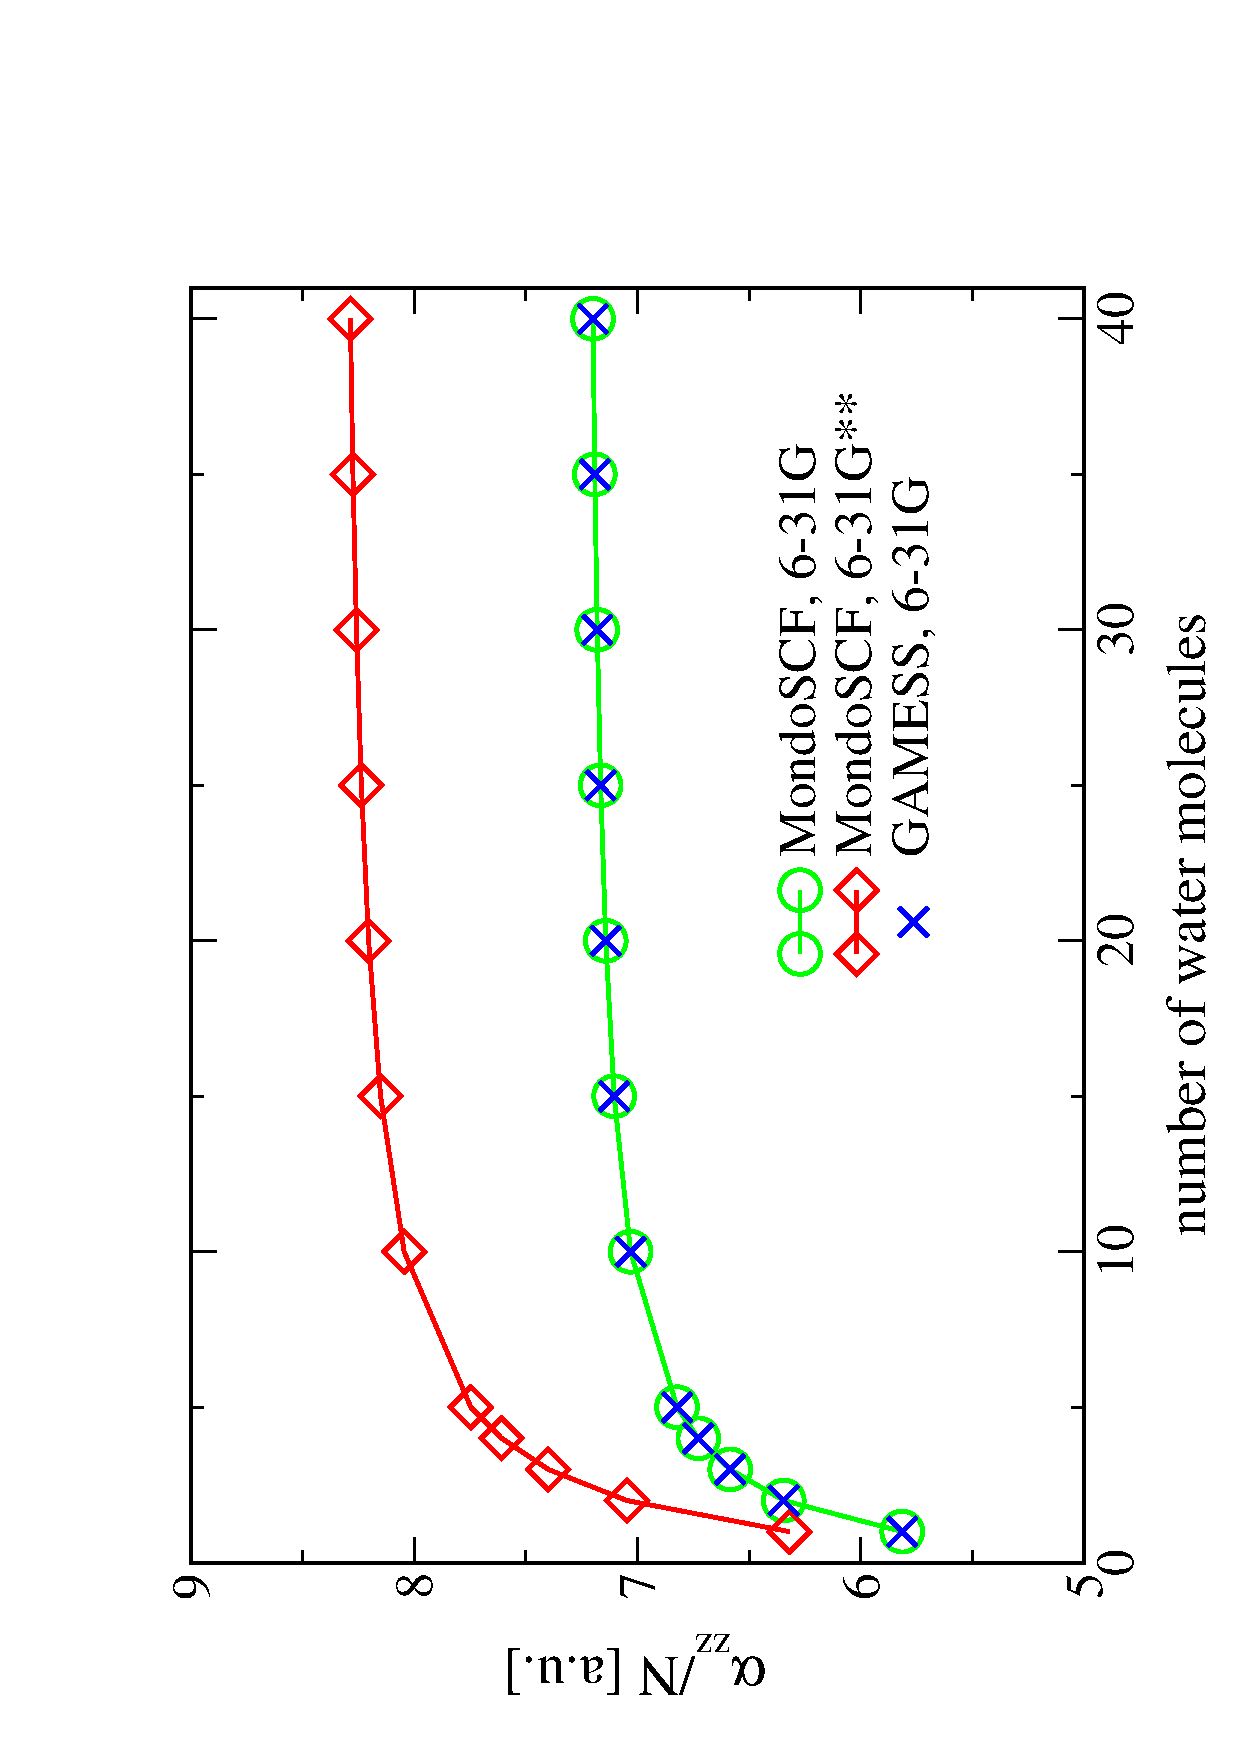
\includegraphics[angle=-90.00]
                       {Alpha_all}}
%                       {Alpha_All}}
\end{figure}


\begin{figure}[t]
  \caption{\protect
    Longitudinal first hyperpolarizability per water 
    molecule $\beta_{zzz}/N$ for 
    the 6-31G and 6-31G** basis sets in function
    of the number of water molecule in the chain.
  }\label{fig:Beta_1D}
  \resizebox*{3.6in}{!}{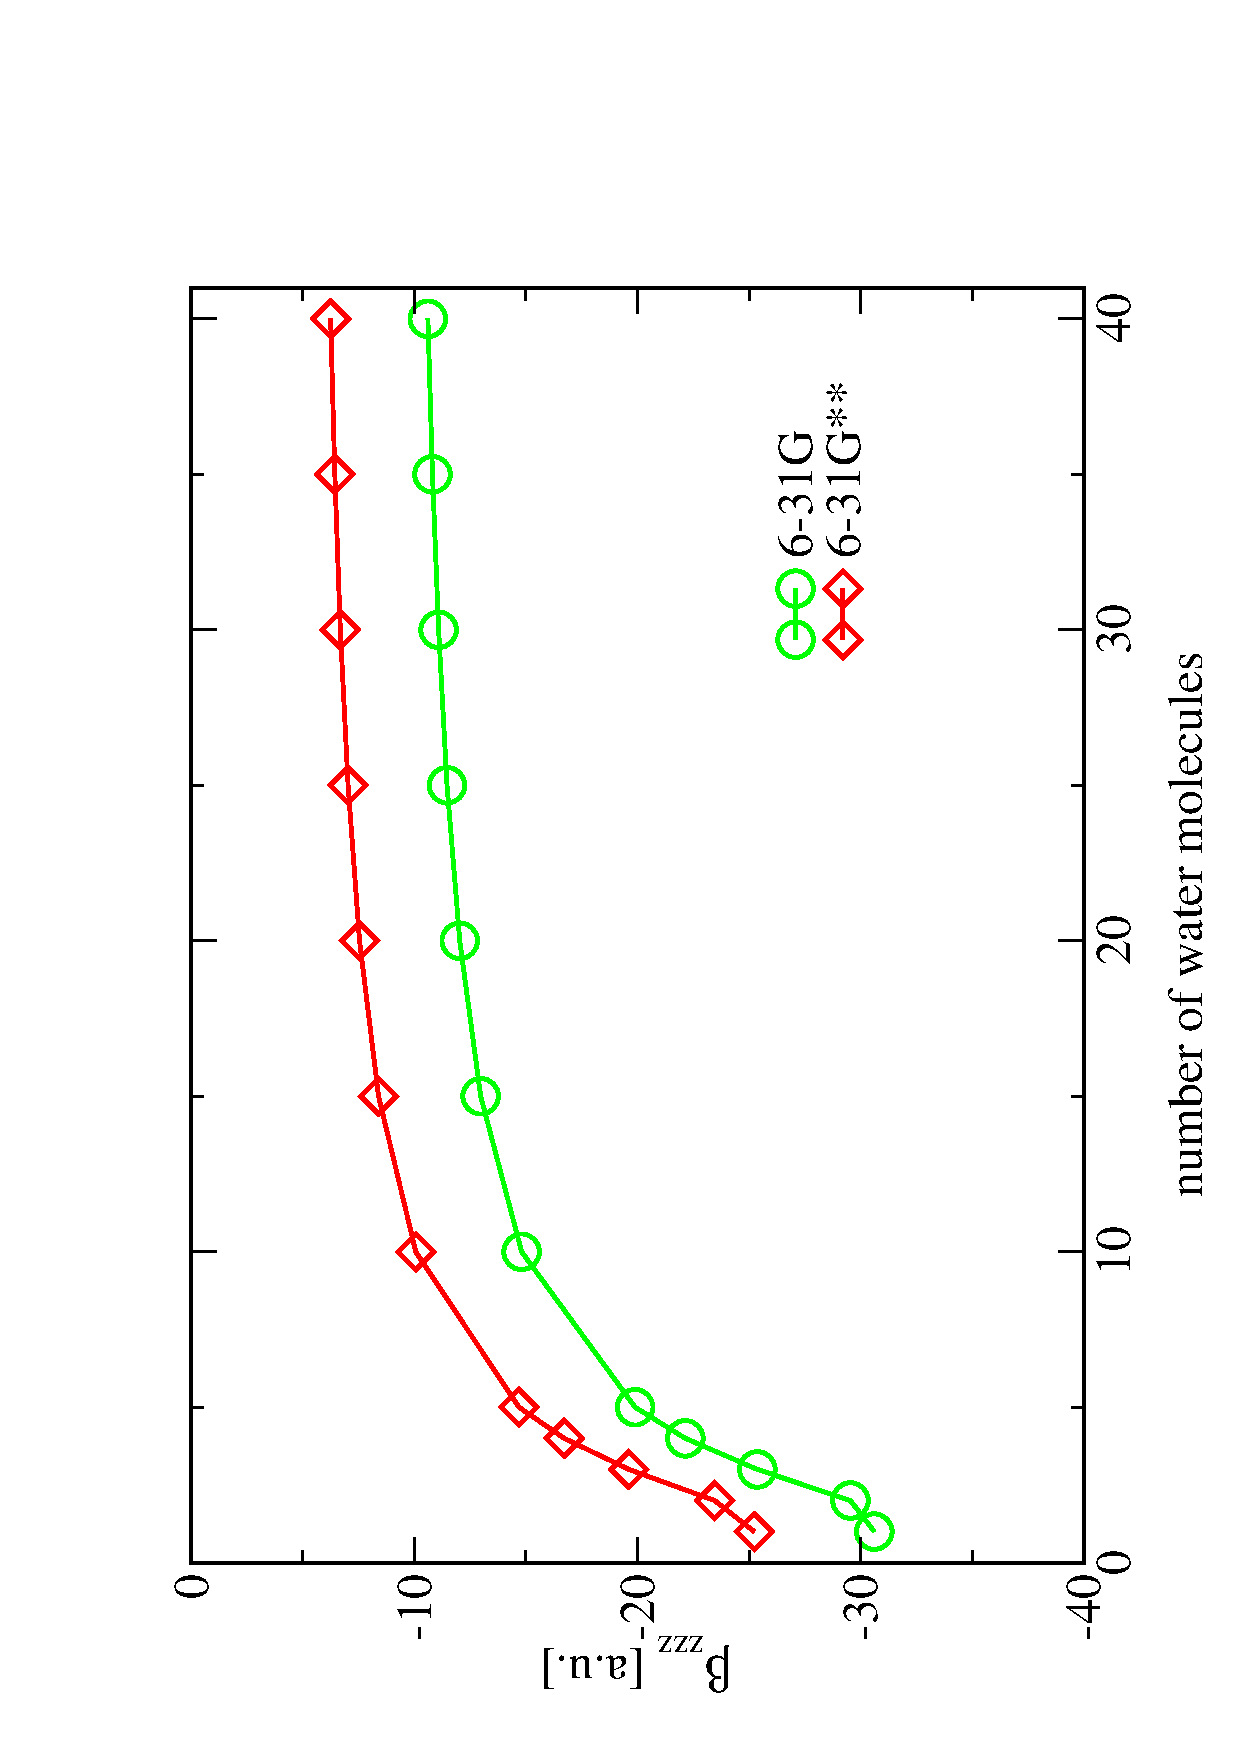
\includegraphics[angle=-90.00]
                       {Beta_all}}
%                       {Beta_All}}
\end{figure}


\begin{figure}[t]
  \caption{\protect
    Longitudinal second hyperpolarizability per water
    molecule $\gamma_{zzzz}/N$ for 
    the 6-31G and 6-31G** basis sets in function
    of the number of water molecule in the chain.
  }\label{fig:Gamma_1D}
  \resizebox*{3.6in}{!}{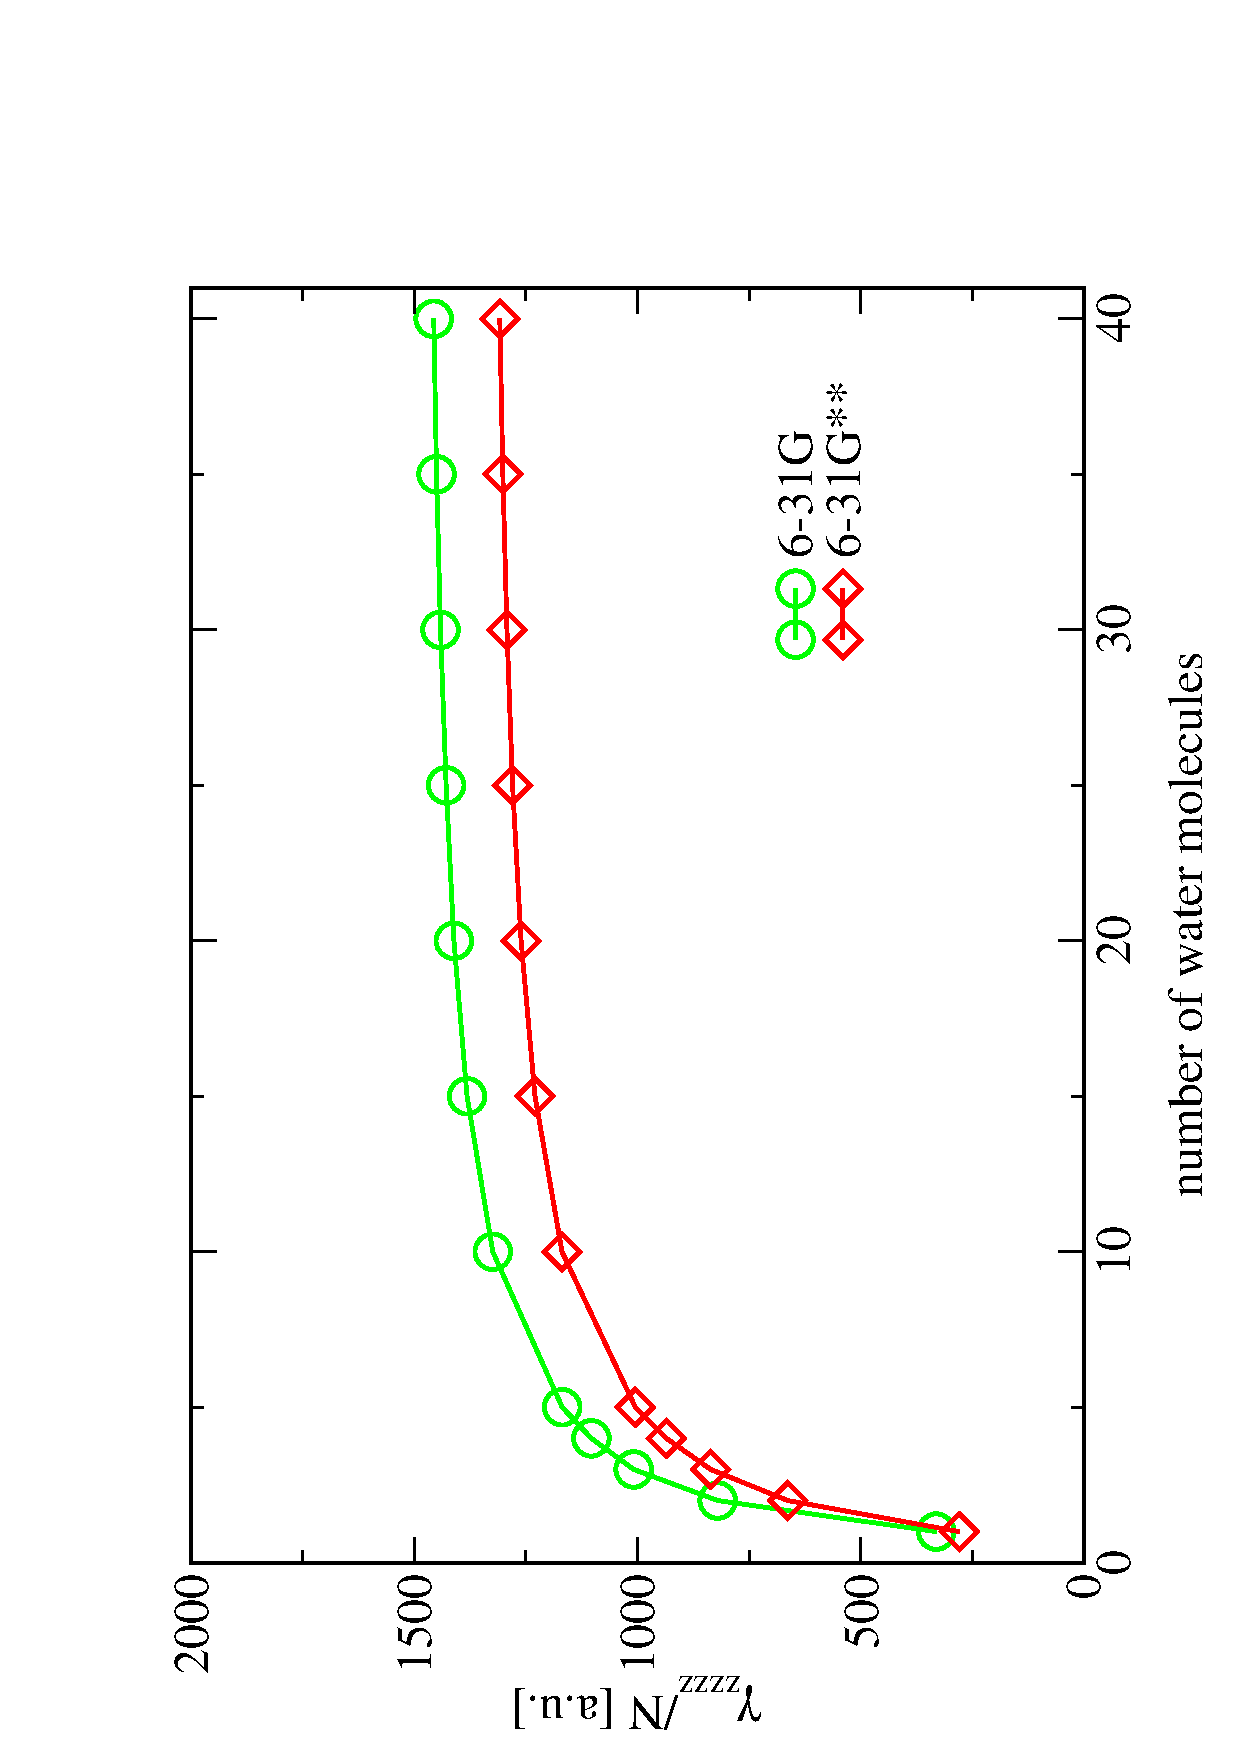
\includegraphics[angle=-90.00]
                       {Gamma_all}}
%                       {Gamma_All}}
\end{figure}


\begin{table}[t]
  \centering
  \caption{\protect
    Longitudinal polarizability $\alpha_{zz}$
    for different water chain lengths with the 6-31G and 6-31G** basis sets
    and {\tt TIGHT} accuracy (See text) and the results obtained with
    the GAMESS quantum chemistry package \cite{gamess} with the 6-31G. 
    All the results are in $[a.u.]$.
    WE CAN REMOVE SOME DIGITS.
  }\label{tab:Alpha_1D_Values}
  \begin{tabular}{cccc}
    \toprule
    $N$ &\multicolumn{1}{c}{6-31G\footnote[1]{\sc GAMESS.}}
        &\multicolumn{1}{c}{6-31G\footnote[2]{\sc MondoSCF.}}
        &\multicolumn{1}{c}{6-31G**$^b$}\\
    \hline
     1 & 5.8136 & 5.813589 & 6.318837     \\
     2 & 6.3448 & 6.344830 & 7.047412     \\
     3 & 6.5844 & 6.584449 & 7.399737     \\
     4 & 6.7276 & 6.727684 & 7.609261     \\
     5 & 6.8226 & 6.822640 & 7.746704     \\
    10 & 7.0308 & 7.030870 & 8.045561     \\
    15 & 7.1047 & 7.104780 & 8.151306     \\
    20 & 7.1424 & 7.142433 & 8.205162     \\
    25 & 7.1652 & 7.165231 & 8.237774     \\
    30 & 7.1805 & 7.180514 & 8.259633     \\
    35 & 7.1914 & 7.191468 & 8.275303     \\
    40 & 7.1996 & 7.199704 & 8.287090     \\
    \botrule
  \end{tabular}
\end{table}


\begin{table}
  \centering
  \caption{\protect
    Longitudinal first hyperpolarizability $\beta_{zzz}$
    for different water chain lengths with the 6-31G and 6-31G** basis sets
    and {\tt TIGHT} accuracy (See text) and the results obtained with
    the GAMESS quantum chemistry package \cite{gamess} with the 6-31G. 
    All the results are in $[a.u.]$.
    WE CAN REMOVE SOME DIGITS.
  }\label{tab:Beta_1D_Values}
  \begin{tabular}{ccccc}
    \toprule
    $N$ &\multicolumn{1}{c}{6-31G\footnote[1]{\sc GAMESS.}}
    &\multicolumn{1}{c}{6-31G\footnote[2]{\sc MondoSCF.}}
    &\multicolumn{1}{c}{6-31G$^{b,}$
      \footnote[3]{The density matrix based 2n+1 rule has been used.}}
    &\multicolumn{1}{c}{6-31G**}$^b$ \\
    \hline
     1 & -30.6125 & -30.612178 & -30.612274 & -25.232854 \\
     2 & -29.5444 & -29.545096 & -29.545207 & -23.454776 \\
     3 & -25.3696 & -25.370516 & -25.370628 & -19.611398 \\
     4 & -22.1411 & -22.141553 & -22.141869 & -16.713840 \\
     5 & -19.8925 & -19.893306 & -19.893441 & -14.683861 \\
    10 & -14.8063 & -14.807203 & -14.807392 & -10.065481 \\
    15 & -12.9713 & -12.972171 & -12.972379 &  -8.396753 \\
    20 & -12.0334 & -12.034259 & -12.034505 &  -7.544200 \\
    25 & -11.4648 & -11.465624 & -11.465915 &  -7.027523 \\
    30 & -11.0834 & -11.084234 & -11.084569 &  -6.680997 \\
    35 & -10.8099 & -10.810645 & -10.811061 &  -6.432514 \\
    40 & -10.6042 & -10.604860 & -10.605360 &  -6.245644 \\
    \botrule
  \end{tabular}
\end{table}


\begin{table}
  \centering
  \caption{\protect
    Longitudinal second hyperpolarizability $\gamma_{zzzz}$
    for different water chain lengths with the 6-31G and 6-31G** basis sets
    and {\tt TIGHT} accuracy (See text) and the results obtained with
    the GAMESS quantum chemistry package \cite{gamess} with the 6-31G. 
    All the results are in $[a.u.]$.
    WE CAN REMOVE SOME DIGITS.
  }\label{tab:Gamma_1D_Values}
  \begin{tabular}{ccccc}
    \toprule
    $N$ &\multicolumn{1}{c}{6-31G\footnote[1]{\sc GAMESS.}}
    &\multicolumn{1}{c}{6-31G\footnote[2]{\sc MondoSCF.}}
    &\multicolumn{1}{c}{6-31G$^{b,}$
      \footnote[3]{The density matrix based 2n+1 rule has been used.}}
    &\multicolumn{1}{c}{6-31G**}$^b$ \\
    \hline
     1 &  330.5753 &  330.577009 &  330.572592 &  278.898509 \\
     2 &  820.1398 &  820.160650 &  820.153734 &  663.493200 \\
     3 & 1008.5656 & 1008.580733 & 1008.582556 &  836.073966 \\
     4 & 1103.4813 & 1103.494950 & 1103.497148 &  935.378474 \\
     5 & 1168.9563 & 1168.972479 & 1168.975145 & 1004.896120 \\
    10 & 1324.2906 & 1324.304700 & 1324.307818 & 1169.020999 \\
    15 & 1381.8657 & 1381.882600 & 1381.882180 & 1229.747000 \\
    20 & 1411.4264 & 1411.448699 & 1411.437607 & 1260.928449 \\
    25 & 1429.3767 & 1428.980999 & 1429.379837 & 1279.877079 \\
    30 & 1441.4261 & 1441.474333 & 1441.418800 & 1292.603933 \\
    35 & 1450.0713 & 1450.143685 & 1450.043351 & 1301.746485 \\
    40 & 1456.5756 & 1456.682800 & 1456.520170 & 1308.644675 \\
    \botrule
  \end{tabular}
\end{table}



\subsection{Linear scaling: 3D water clusters}


Calculations have been carried out at both the RHF/6-31G and RHF/6-31G** levels of
theory and at both the {\tt GOOD} and {\tt TIGHT} thresholding parameter 
sets that control precision of the linear scaling algorithms, corresponding 
to matrix thresholds of $10^{-5}$ and $10^{-6}$, respectively.

3D water clusters show an early onset of linear scaling for accurate
basis set and low thresholds and higher order response.


\subsection{Exponential decay}
Figure \ref{fig:Superposition_Decay} shows the superposition 
of the magnitude of density matrix derivative atom-atom blocks up to 
third order as a function of atom-atom distance when perturbed by 
a static electric field. 
The density responses matrices show an exponential decay as a function
of the internuclear distance, however the decay is slower and the locality
becomes lower for the higher order response functions.
Therefor, we find a later onset for the linear scaling for the higher order
responses. 



\begin{figure}[t]
  \caption{\protect
    Total WALL time of the fifth first order CPSCF iteration for
    the water cluster sequence with the 6-31G and 6-31G** 
    basis sets and the {\tt GOOD} and {\tt TIGHT} 
    numerical thresholds (see text) controlling numerical
    precision of the result. The lines are fits to the 
    last three and four points, respectively.
  }\label{Alpha_scaling}
  \resizebox*{3.6in}{!}{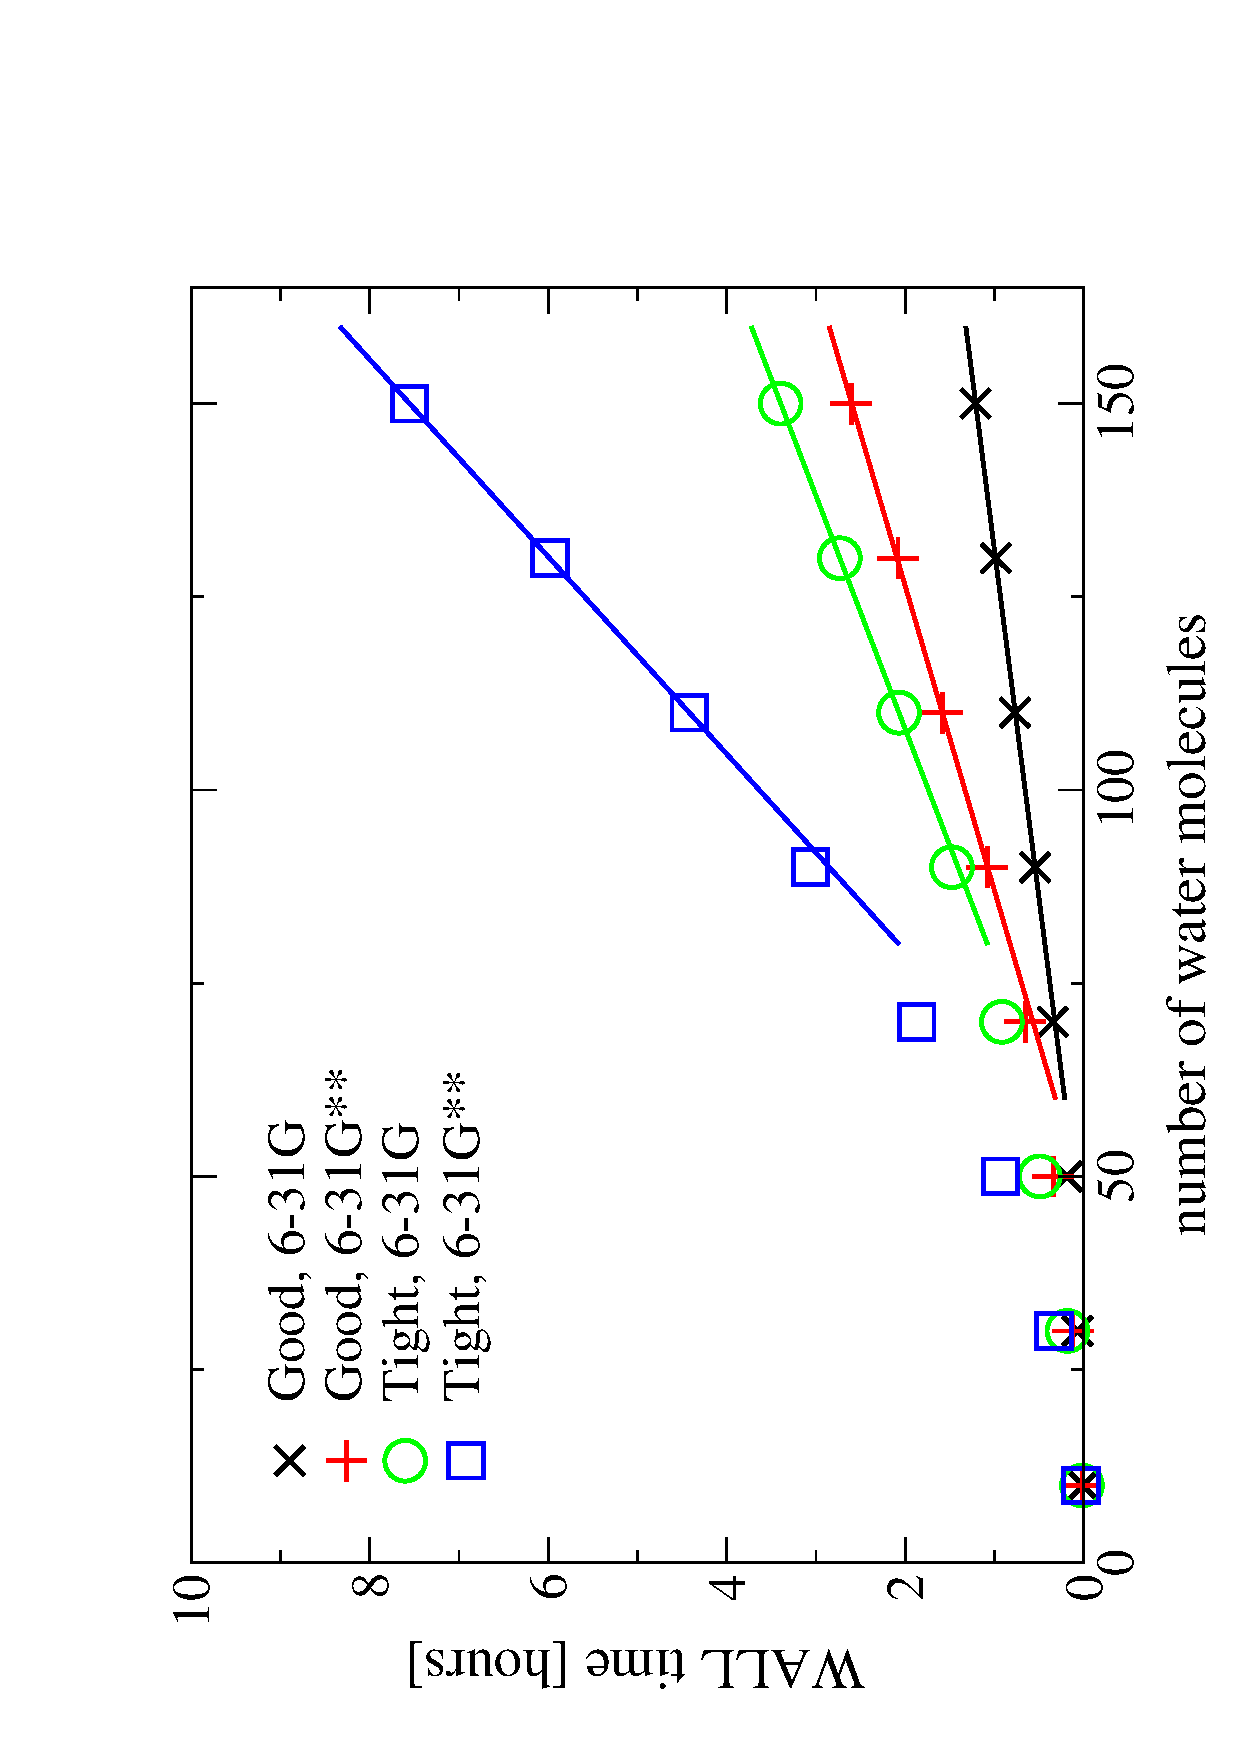
\includegraphics[angle=-90.00]
                        {Alpha_h2o3D_6-31G_6-31Gss_G_T}}
%                        {Alpha_h2o3D_6-31G_6-31Gss_G_T_t}}
\end{figure}


\begin{figure}[t]
  \caption{\protect
    Total WALL time of the fifth second order CPSCF iteration for
    the water cluster sequence with the 6-31G and 6-31G** 
    basis sets and the {\tt GOOD} and {\tt TIGHT} 
    numerical thresholds (see text) controlling numerical
    precision of the result. The lines are fits to the 
    last three and four points, respectively.
  }\label{Beta_scaling}
  \resizebox*{3.6in}{!}{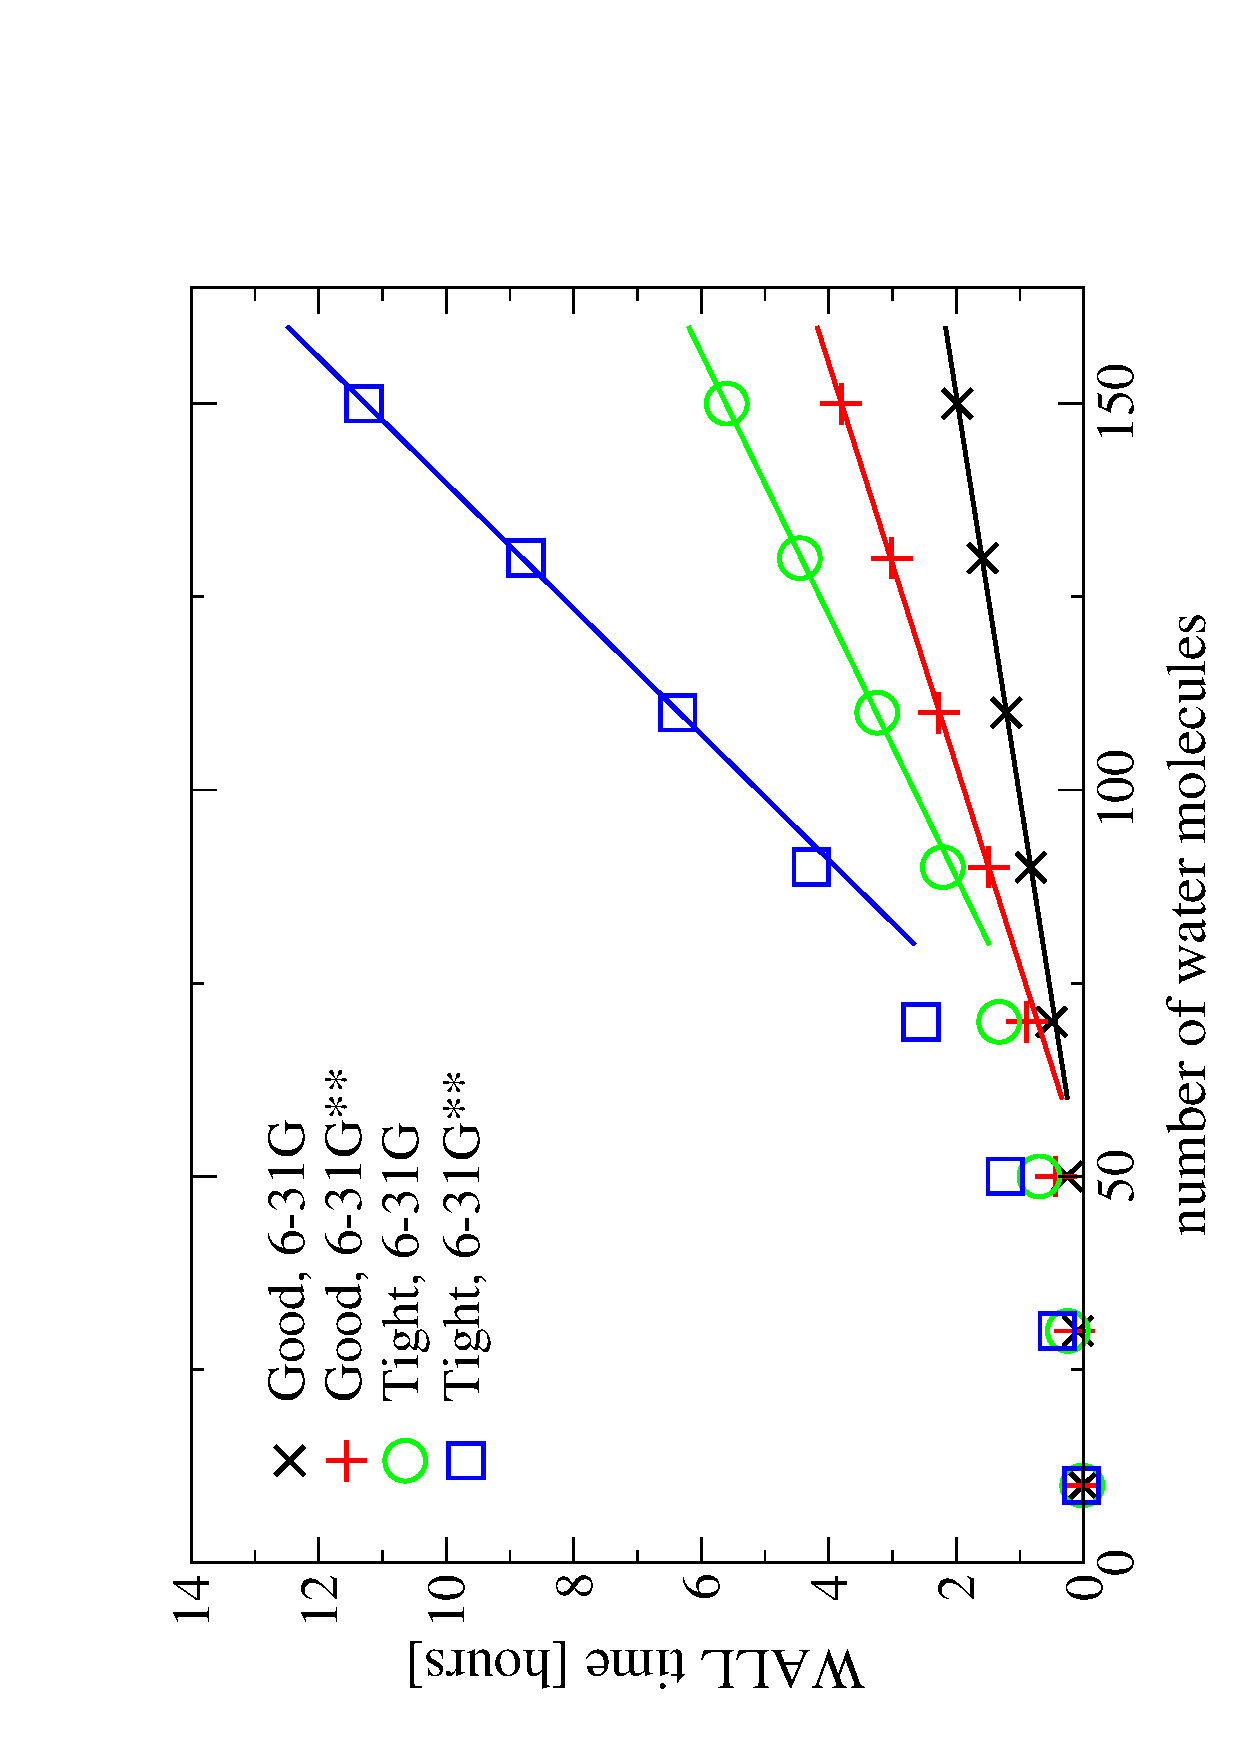
\includegraphics[angle=-90.00]
                        {Beta_h2o3D_6-31G_6-31Gss_G_T}}
%                        {Beta_h2o3D_6-31G_6-31Gss_G_T_t}}
\end{figure}


\begin{figure}[t]
  \caption{\protect
    Total WALL time of the fifth third order CPSCF iteration for
    the water cluster sequence with the 6-31G and 6-31G** 
    basis sets and the {\tt GOOD} and {\tt TIGHT} 
    numerical thresholds (see text) controlling numerical
    precision of the result. The lines are fits to the 
    last three and four points, respectively.
  }\label{Gamma_scaling}
  \resizebox*{3.6in}{!}{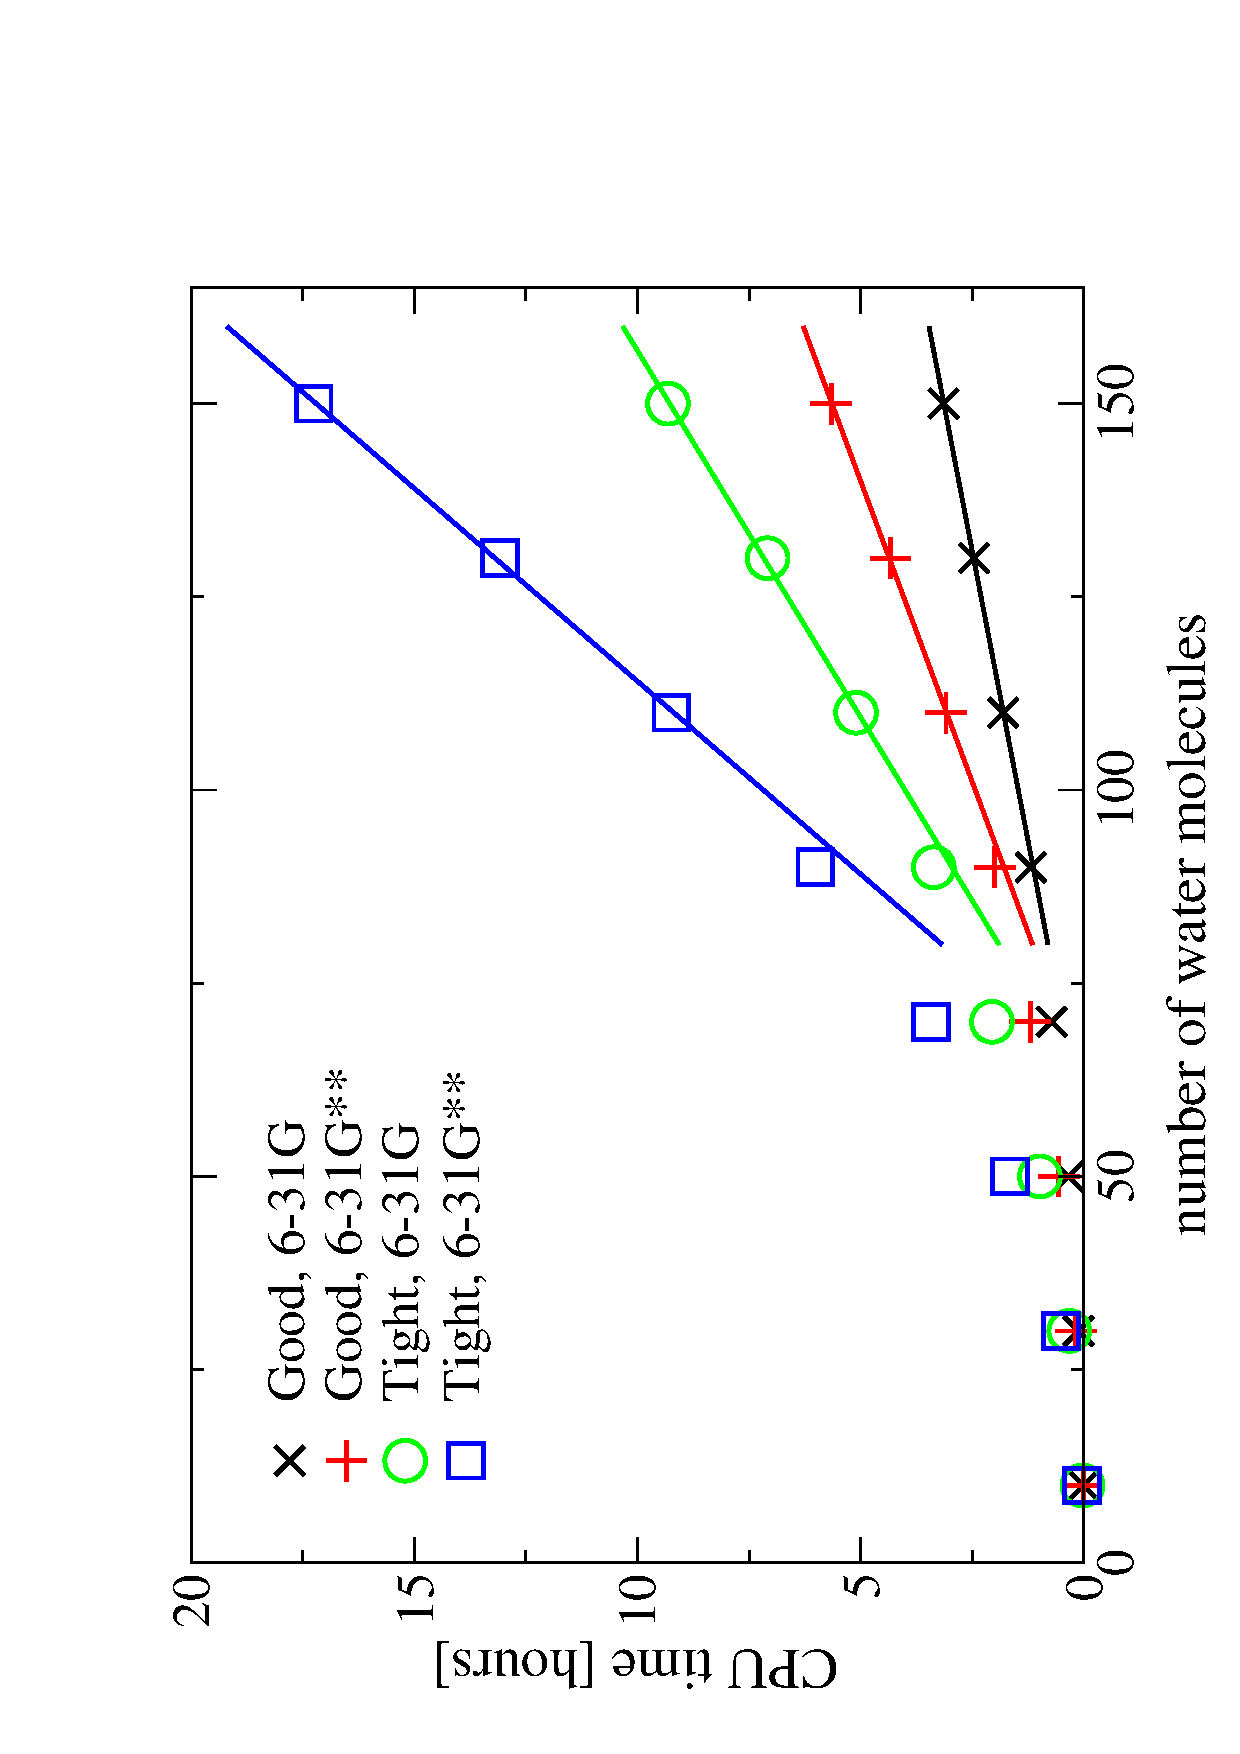
\includegraphics[angle=-90.00]
                        {Gamma_h2o3D_6-31G_6-31Gss_G_T}}
%                        {Gamma_h2o3D_6-31G_6-31Gss_G_T_t}}
\end{figure}



\begin{figure}[t]
  \caption{\protect
    Total WALL time of the fifth first, second and third order
    CPSCF iteration for the water cluster sequence with the 6-31G
    basis set and the {\tt TIGHT} numerical threshold (see text) 
    controlling numerical precision of the result. The lines
    are fits to the last three and four points, respectively.
  }\label{Mix_scaling}
  \resizebox*{3.6in}{!}{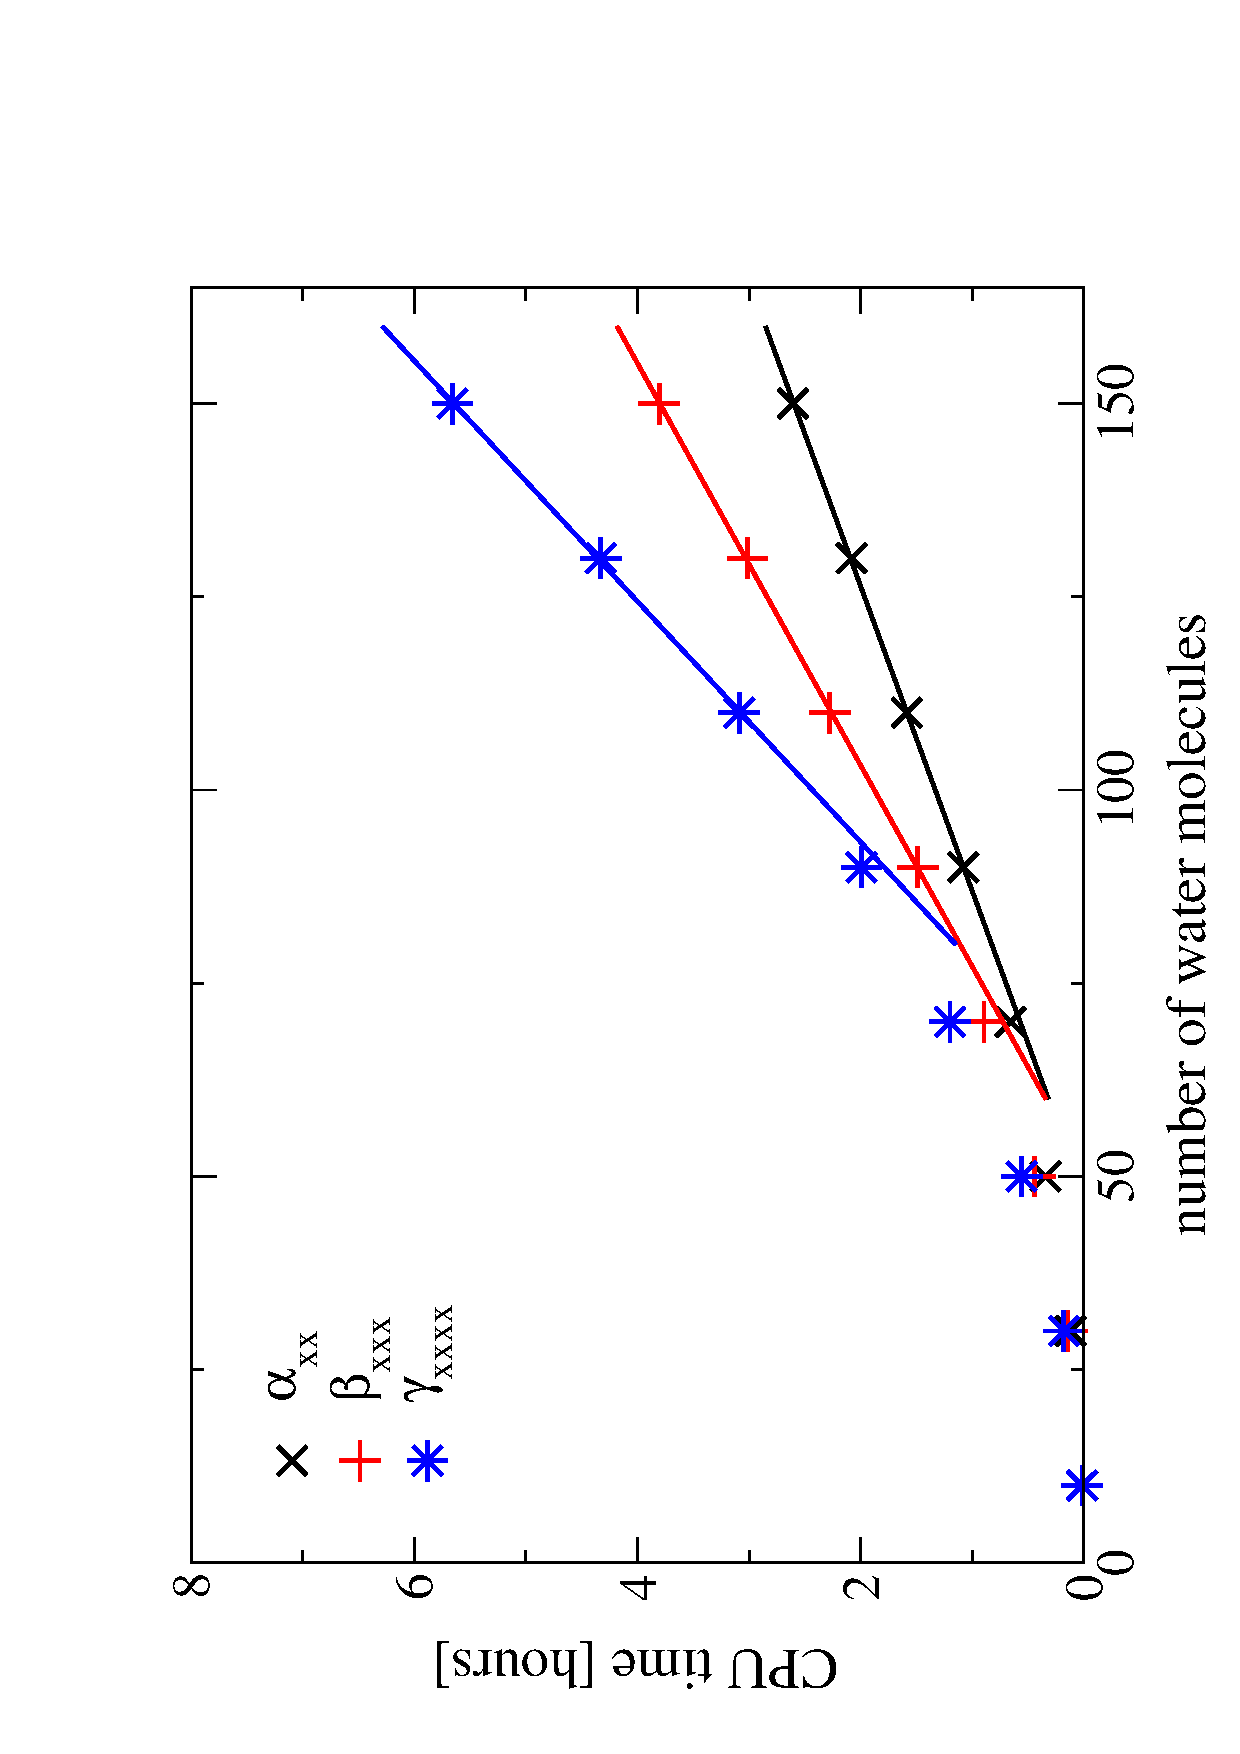
\includegraphics[angle=-90.00]
                        {Mix_h2o3D_6-31G_T}}
%                        {Mix_h2o3D_6-31G_6-31Gss_G_T_t}}
\end{figure}


\begin{figure}[t]
  \caption{\protect
    TC2R WALL time of the fifth third order CPSCF iteration for
    the water cluster sequence with the 6-31G and 6-31G** 
    basis sets and the {\tt GOOD} and {\tt TIGHT} 
    numerical thresholds (see text) controlling numerical
    precision of the result. The lines are fits to the 
    last three and four points, respectively.
  }\label{fig:Gamma_TC2R_Timing}
  \resizebox*{3.6in}{!}{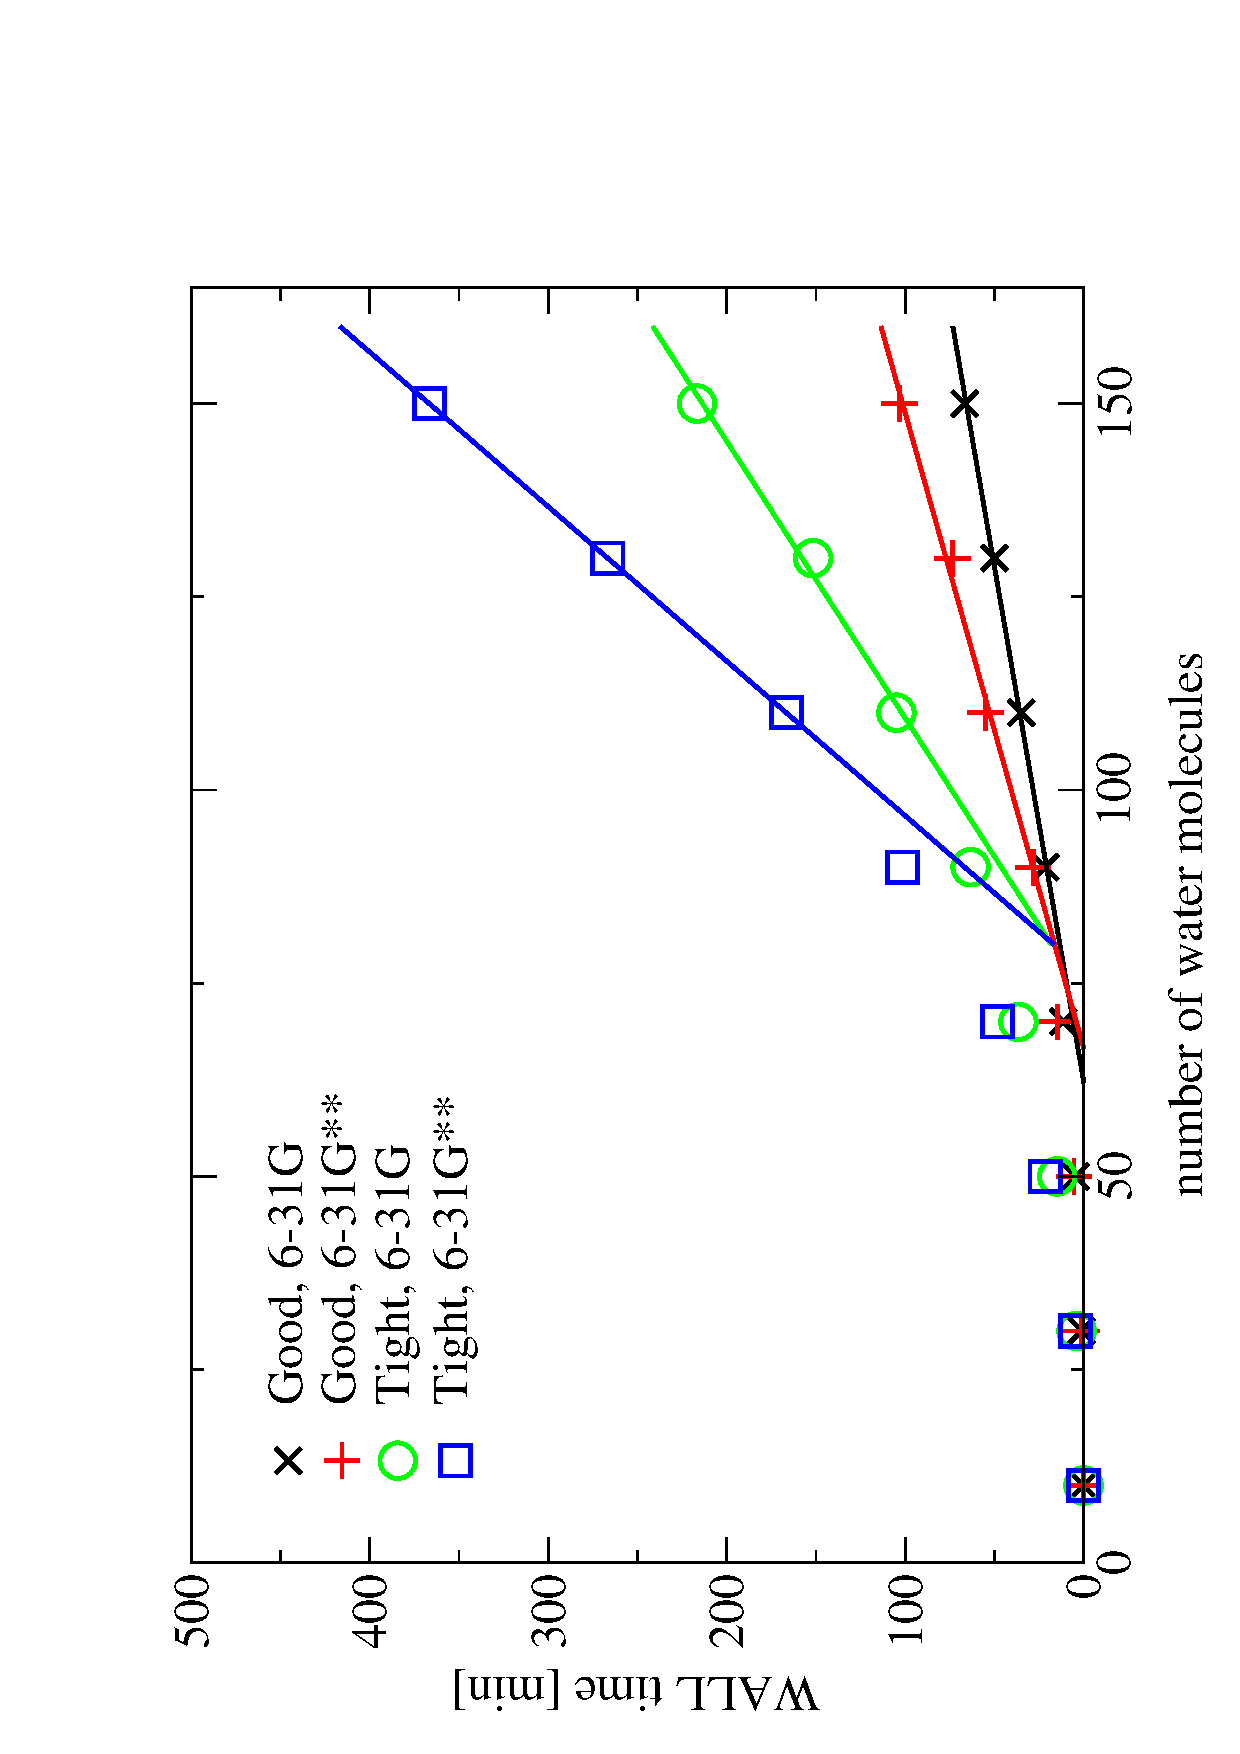
\includegraphics[angle=-90.00]{Gamma_TC2R_T}}
\end{figure}


\begin{figure}[t]
  \caption{\protect
    QCTC WALL time of the fifth third order CPSCF iteration for
    the water cluster sequence with the 6-31G and 6-31G** 
    basis sets and the {\tt GOOD} and {\tt TIGHT} 
    numerical thresholds (see text) controlling numerical
    precision of the result. The lines are fits to the 
    last three and four points, respectively.
  }\label{fig:Gamma_QCTC_Timing}
  \resizebox*{3.6in}{!}{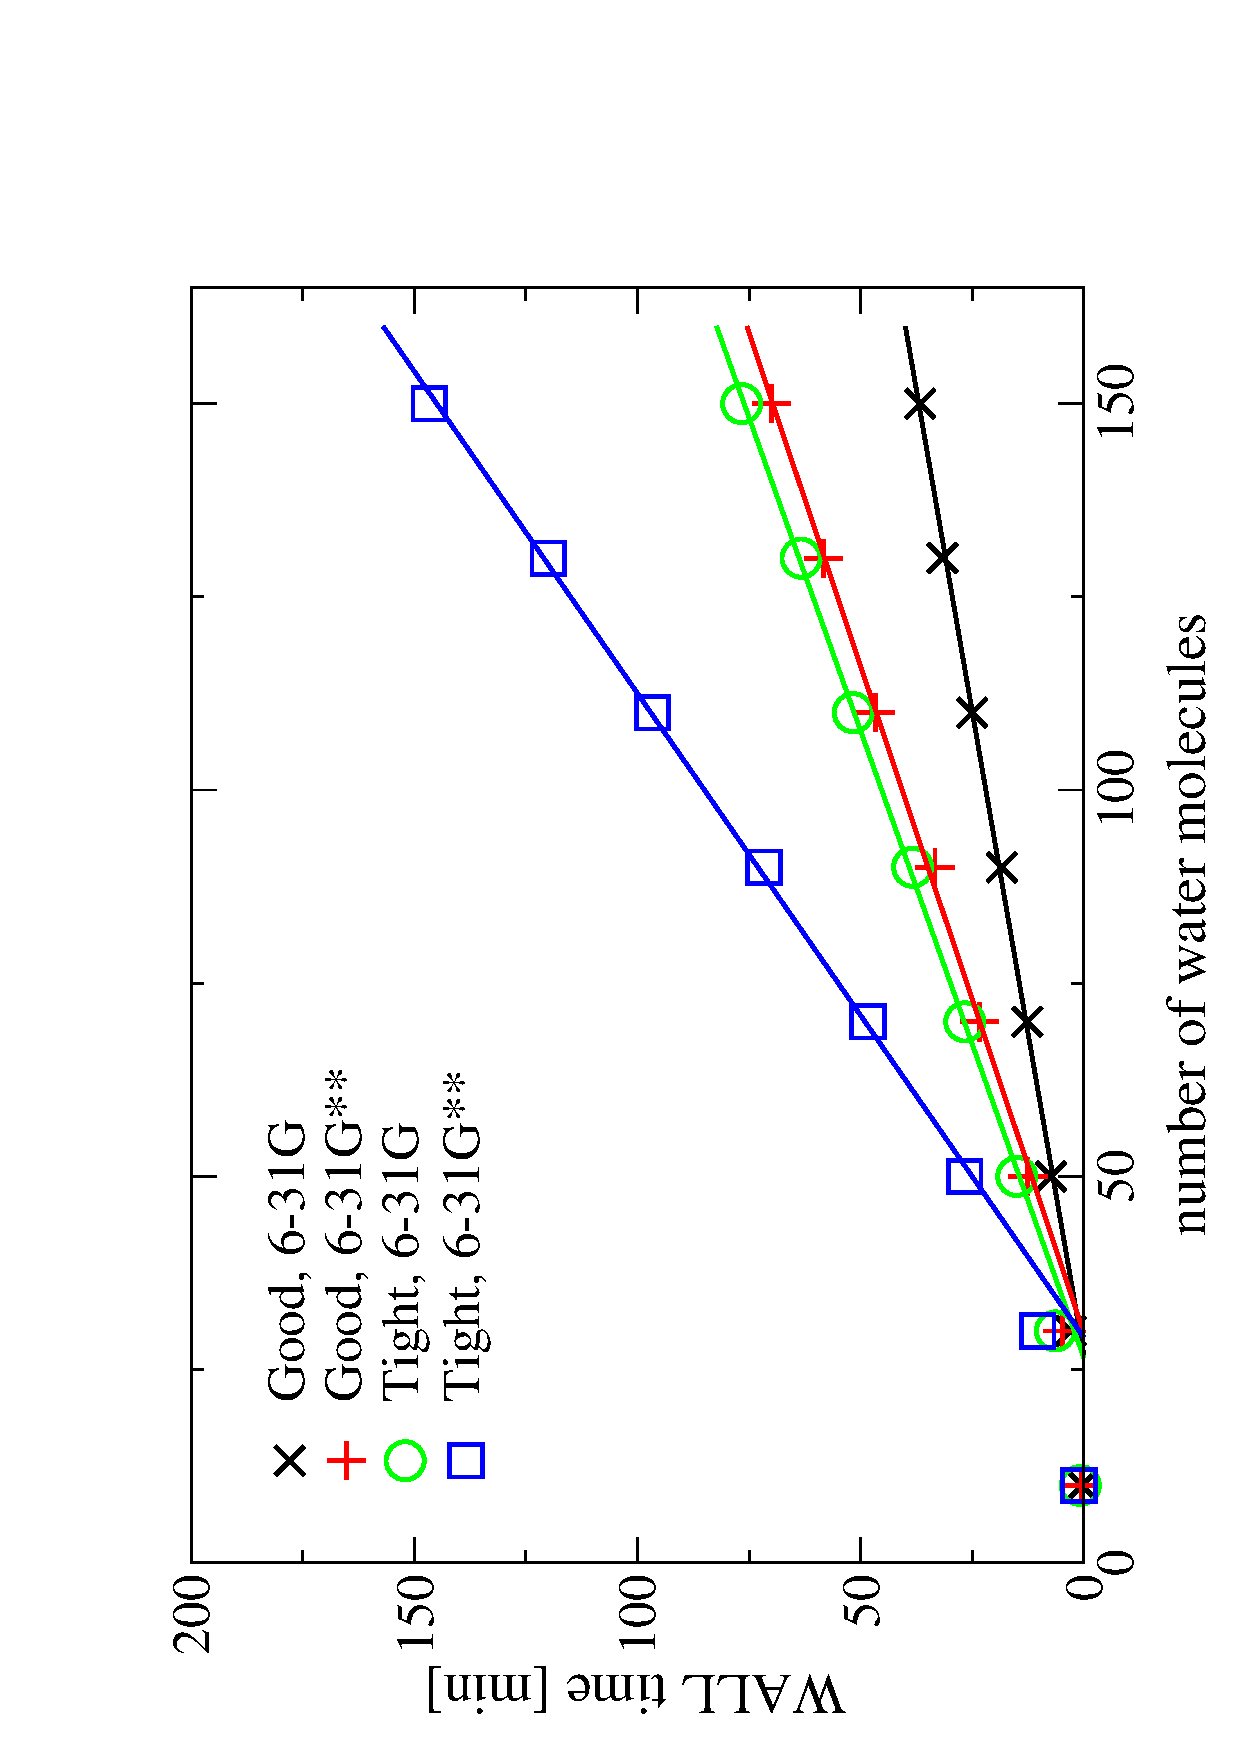
\includegraphics[angle=-90.00]{Gamma_QCTC_T}}
\end{figure}


\begin{figure}[t]
  \caption{\protect
    ONX WALL time of the fifth third order CPSCF iteration for
    the water cluster sequence with the 6-31G and 6-31G** 
    basis sets and the {\tt GOOD} and {\tt TIGHT} 
    numerical thresholds (see text) controlling numerical
    precision of the result. The lines are fits to the 
    last three and four points, respectively.
  }\label{fig:Gamma_ONX_Timing}
  \resizebox*{3.6in}{!}{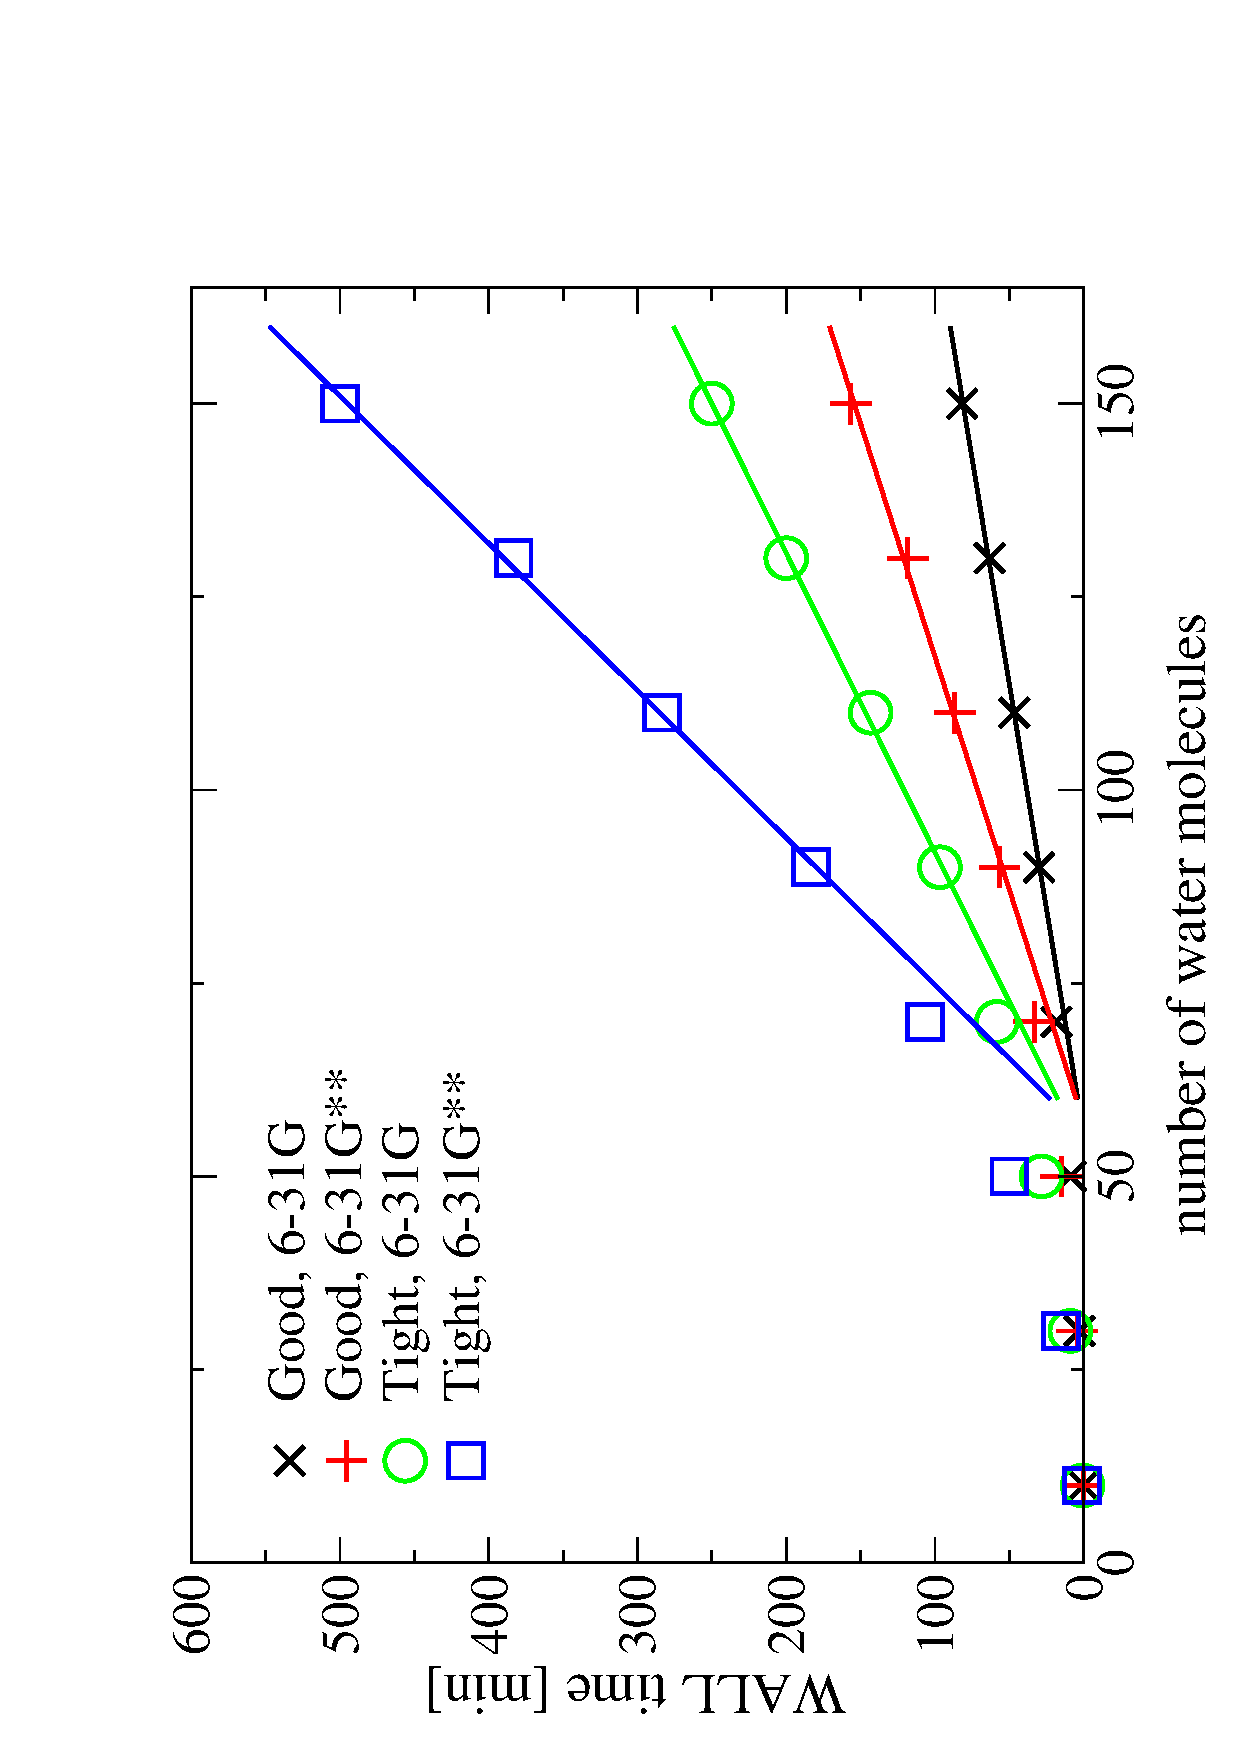
\includegraphics[angle=-90.00]{Gamma_ONX_T}}
\end{figure}




%\begin{figure}[t]
%  \caption{\protect
%    WE MAY REMOVE THIS!
%    Magnitudes of the RHF/6-31G density matrix derivative elements $D^{x}_{cd}$
%    along the $x$ axis with the separation of basis function centers
%    for the $\rm (H_2O)_{150}$ water cluster. The density matrix 
%    derivative has been converged to within {\tt TIGHT} (e.g. 
%    matrix threshold of $10^{-6}$ $[a.u.]$).
%  }\label{fig:Alpha_Decay}
%  %  \resizebox*{3.5in}{!}{\includegraphics[angle=-90.00]{}}
%\end{figure}


%\begin{figure}[t]
%  \caption{\protect
%    WE MAY REMOVE THIS!
%    Magnitudes of the RHF/6-31G density matrix second derivative elements $D^{xx}_{cd}$
%    along the $x$ axis with the separation of basis function centers
%    for the $\rm (H_2O)_{150}$ water cluster. The density matrix 
%    derivative has been converged to within {\tt TIGHT} (e.g. 
%    matrix threshold of $10^{-6}$ $[a.u.]$).
%  }\label{fig:Beta_Decay}
%  %  \resizebox*{3.5in}{!}{\includegraphics[angle=-90.00]{}}
%\end{figure}


%\begin{figure}[t]
%  \caption{\protect
%    WE MAY REMOVE THIS!
%    Magnitudes of the RHF/6-31G density matrix third derivative elements $D^{xxx}_{cd}$
%    along the $x$ axis with the separation of basis function centers
%    for the $\rm (H_2O)_{150}$ water cluster. The density matrix 
%    derivative has been converged to within {\tt TIGHT} (e.g. 
%    matrix threshold of $10^{-6}$ $[a.u.]$).
%  }\label{fig:Beta_Decay}
%  %  \resizebox*{3.5in}{!}{\includegraphics[angle=-90.00]{}}
%\end{figure}


\begin{figure}[t]
  \caption{\protect
    Superposition of the magnitudes of the RHF/6-31G density matrix
    derivative elements $D_{cd}$, $D^{x}_{cd}$, $D^{xx}_{cd}$ and $D^{xxx}_{cd}$
    along the $x$ axis with the separation of basis function centers
    for the $\rm (H_2O)_{150}$ water cluster. The density matrix 
    derivatives have been converged to within {\tt TIGHT} (e.g. 
    matrix threshold of $10^{-6}$ $[a.u.]$).
    IT MISS THE GROUND STATE DENSITY MATRIX.
  }\label{fig:Superposition_Decay}
  \resizebox*{3.5in}{!}{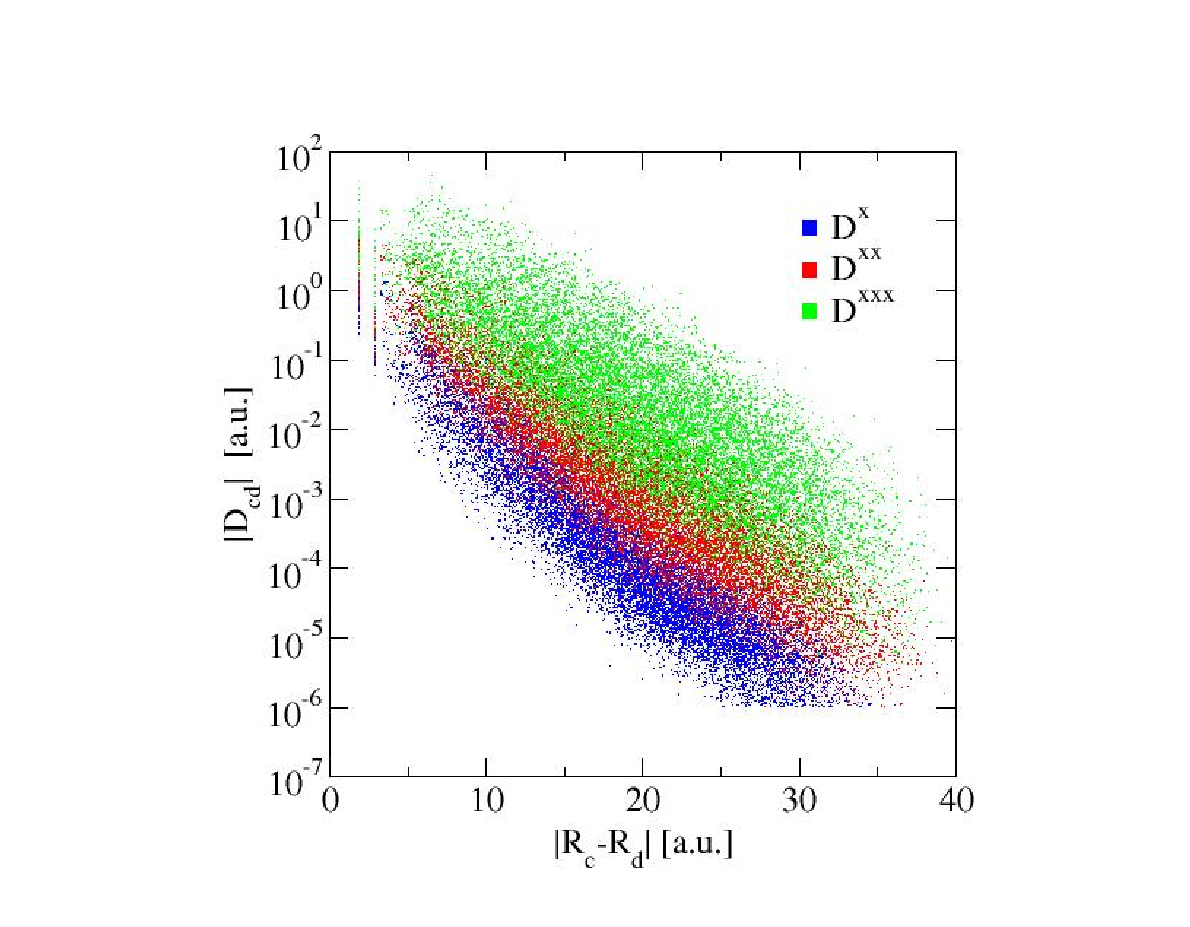
\includegraphics[angle=0.00]{DPrimeMix2}}
\end{figure}




%%%%%%%%%%%%%%%%%%%%%%%%%%%%%%%%%%%%%%%%%%%%%%%%%%%%%%%%%%%%%%%%
%%%%%%%%%%%%%%%%%%%%%%%%%%%%%%%%%%%%%%%%%%%%%%%%%%%%%%%%%%%%%%%%
\section{Summary and Conclusion}


 We have proposed and demonstrated a linear scaling self
 consistent scheme for high order response properties.
 The scheme solves the coupled perturbed self consistent field 
 equation by the perturbed projection method. We have also shown
 that the perturbed projection method can be expended to high
 order (e.g. up to 10-th order in the present paper).

We have presented a simple and efficient algorithm for solution 
of the coupled-perturbed self-consistent-field (CPSCF) equations 
in the context of spectral projection and static
electric polarizabilities. Unique features of the perturbed 
projection algorithm include linear scaling, simplicity, numerical 
stability and quadratic convergence in computation of the derivative
density matrices.

We have shown that the density matrix response is local 
upon {\em global} electric perturbation, corresponding to an approximate 
exponential decay of matrix elements. A similar exponential decay
in the first order response corresponding to the {\em local} nuclear 
displacement has previously been demonstrated by Ochsenfeld and 
Head-Gordon \cite{Ochsenfeld_1997}. These key observations are expected to
hold generally for both local and global perturbations to insulating systems.  
We note also that the method is not unique to the TC2 generator or 
{\sc MondoSCF} $N$-scaling algorithms, but can be straightforwardly 
extended to other purification schemes such as TRS4 \cite{ANiklasson03} as
well as other electronic structure programs.

Convergence of the CPSCF equations for these systems (water cluster ...)
are typically achived in about 10 cycles, independent of cluster size, basis set,
matrix threshold or order of the response calculated.

%%%%%%%%%%%%%%%%%%%%%%%%%%%%%%%%%%%%%%%%%%%%%%%%%%%%%%%%%%%%%%%%
%%%%%%%%%%%%%%%%%%%%%%%%%%%%%%%%%%%%%%%%%%%%%%%%%%%%%%%%%%%%%%%%
%Acknowledgements
\begin{acknowledgments}
 This work has been supported by the US Department of Energy 
 under contract ???????????? and the ASCI project.  
 The Advanced Computing Laboratory of Los 
 Alamos National Laboratory is acknowledged.
 All the numerical computations have been
 performed on computing resources located at this facility.
\end{acknowledgments}
%%%%%%%%%%%%%%%%%%%%%%%%%%%%%%%%%%%%%%%%%%%%%%%%%%%%%%%%%%%%%%%%
%%%%%%%%%%%%%%%%%%%%%%%%%%%%%%%%%%%%%%%%%%%%%%%%%%%%%%%%%%%%%%%%
\bibliography{Response3}
%%%%%%%%%%%%%%%%%%%%%%%%%%%%%%%%%%%%%%%%%%%%%%%%%%%%%%%%%%%%%%%%
%%%%%%%%%%%%%%%%%%%%%%%%%%%%%%%%%%%%%%%%%%%%%%%%%%%%%%%%%%%%%%%%
%%%%%%%%%%%%%%%%%%%%%%%%%%%%%%%%%%%%%%%%%%%%%%%%%%%%%%%%%%%%%%%%
%%%%%%%%%%%%%%%%%%%%%%%%%%%%%%%%%%%%%%%%%%%%%%%%%%%%%%%%%%%%%%%%
%%%%%%%%%%%%%%%%%%%%%%%%%%%%%%%%%%%%%%%%%%%%%%%%%%%%%%%%%%%%%%%%
\end{document}
%
% ****** End of file apssamp.tex ******
